% ============================================================================
% Trabajo Práctico Final — Deep Learning
% Sistema de Detección y Segmentación de Objetos en Tiempo Real
% Autor: Federico Morán
% Compilar con pdflatex (Texmaker: compilación rápida PDFLaTeX, 2 pasadas
% para resolver referencias cruzadas).
% ============================================================================
\documentclass[11pt,a4paper]{article}

\usepackage[utf8]{inputenc}
\usepackage[T1]{fontenc}
\usepackage{lmodern}
\usepackage[spanish,es-tabla]{babel}
\usepackage[margin=2.5cm]{geometry}
\usepackage{graphicx}
\usepackage{booktabs}
\usepackage{amsmath}
\usepackage{float}
\usepackage{caption}
\usepackage{subcaption}
\usepackage{microtype}
\usepackage{listings}
\usepackage{xcolor}
\usepackage[hidelinks]{hyperref}

\graphicspath{{figuras/}}
\captionsetup{font=small,labelfont=bf}

% ---------------------------------------------------------------------------
% Estilo de los listados de código (fragmentos reales del pipeline)
% ---------------------------------------------------------------------------
\definecolor{codebg}{RGB}{247,248,250}
\definecolor{coderule}{RGB}{223,226,230}
\definecolor{codekw}{RGB}{0,72,153}
\definecolor{codestr}{RGB}{163,21,21}
\definecolor{codecom}{RGB}{106,115,125}
\definecolor{codenum}{RGB}{150,150,150}

\renewcommand{\lstlistingname}{Código}

\lstdefinestyle{py}{
  language=Python,
  basicstyle=\ttfamily\scriptsize,
  keywordstyle=\color{codekw}\bfseries,
  stringstyle=\color{codestr},
  commentstyle=\color{codecom}\itshape,
  numberstyle=\color{codenum}\ttfamily\tiny,
  numbers=left, numbersep=7pt,
  backgroundcolor=\color{codebg},
  frame=single, framesep=5pt, rulecolor=\color{coderule},
  breaklines=true, showstringspaces=false, tabsize=2,
  columns=fullflexible, keepspaces=true,
  extendedchars=true, upquote=true,
  aboveskip=1.1em, belowskip=0.6em,
  literate=%
    {á}{{\'a}}1 {é}{{\'e}}1 {í}{{\'i}}1 {ó}{{\'o}}1 {ú}{{\'u}}1
    {Á}{{\'A}}1 {É}{{\'E}}1 {Í}{{\'I}}1 {Ó}{{\'O}}1 {Ú}{{\'U}}1
    {ñ}{{\~n}}1 {Ñ}{{\~N}}1 {¿}{{?`}}1 {¡}{{!`}}1
    {«}{{\guillemotleft{}}}1 {»}{{\guillemotright{}}}1 {°}{{\textdegree}}1,
}

\title{\textbf{Sistema de Detección y Segmentación de Objetos en Tiempo Real
mediante Ajuste Fino de YOLOv8}\\[1ex]
\large Trabajo Práctico Final --- Deep Learning\\
Maestría en Inteligencia Artificial}
\author{Federico Morán}
\date{Julio de 2026}

\begin{document}

\maketitle

\begin{abstract}
\noindent
Este trabajo presenta el desarrollo de un sistema completo de visión por
computadora capaz de detectar y segmentar, en tiempo real, ocho clases de
objetos de entorno doméstico y de oficina. Se construyó un conjunto de datos de
5.000 imágenes y 23.363 instancias anotadas a partir de COCO~2017, se realizó
el ajuste fino (\emph{fine-tuning}) de un modelo de segmentación de instancias
YOLOv8n-seg preentrenado ---con el \emph{backbone} congelado para preservar sus
representaciones--- y se evaluó el resultado sobre una partición de prueba
reservada con las métricas estándar del área, alcanzando un mAP@50-95 de 0,292
para detección (cajas) y 0,246 para segmentación (máscaras). Un aspecto central
del trabajo es el \textbf{rigor de la evaluación}: se identificó que la
comparación directa contra el modelo preentrenado de referencia está sesgada a
su favor, porque dicho modelo fue entrenado sobre el mismo conjunto
(COCO~train2017) del que provienen las imágenes de prueba; para corregirlo se
construyó una evaluación imparcial sobre COCO~val2017, datos que ninguno de los
dos modelos vio durante su entrenamiento. Bajo esa comparación justa la brecha
aparente se reduce a la mitad, y el modelo ajustado (0,236 de mAP@50-95 de
máscaras) se aproxima al preentrenado (0,277), con la ventaja práctica de la
\textbf{especialización}: elimina las detecciones espurias de las 72 categorías
fuera de alcance. El sistema de inferencia, implementado sobre OpenCV con
captura de cámara web, opera a 17~cuadros por segundo sobre una CPU de
consumo, y alcanza 35~cuadros por segundo al optimizar el modelo con OpenVINO,
lo que valida la viabilidad de la segmentación de instancias en tiempo real
sobre hardware no especializado.
\end{abstract}

% ============================================================================
\section{Introducción}

La detección y segmentación de objetos son dos tareas centrales de la visión
por computadora. La \textbf{detección} localiza cada objeto mediante una caja
delimitadora y le asigna una clase; la \textbf{segmentación de instancias} va
un paso más allá y delimita, píxel a píxel, la silueta exacta de cada objeto
individual. Su combinación en un único sistema que opere en \emph{tiempo real}
habilita aplicaciones de robótica, asistencia, control de inventario y
análisis de video, entre otras, pero impone un compromiso exigente entre
precisión y latencia, en particular cuando la inferencia debe ejecutarse sobre
hardware de consumo sin aceleración dedicada.

El objetivo general de este trabajo es desarrollar un sistema completo de
visión por computadora que detecte y segmente objetos en tiempo real. Los
objetivos específicos son: (i)~construir un conjunto de datos supervisado a
partir de COCO~2017; (ii)~ajustar un modelo de segmentación de instancias
mediante transferencia de aprendizaje; (iii)~evaluarlo con las métricas
estándar del área (mAP e IoU, tanto para cajas como para máscaras), incluida
la comparación contra el modelo preentrenado de referencia; y (iv)~implementar
la inferencia en tiempo real sobre una computadora personal, con captura de
cámara web.

El alcance se acotó a ocho clases de objetos de entorno doméstico y de
oficina (\texttt{person}, \texttt{cell phone}, \texttt{cup}, \texttt{bottle},
\texttt{laptop}, \texttt{keyboard}, \texttt{mouse}, \texttt{book}),
seleccionadas con un criterio de aplicación: todas pueden exhibirse
físicamente frente a una cámara web durante la demostración del sistema.

El documento se organiza como sigue. La Sección~\ref{sec:datos} describe la
construcción del conjunto de datos. La Sección~\ref{sec:metodo} presenta la
arquitectura, el preprocesamiento, el aumento de datos y la configuración de
entrenamiento. La Sección~\ref{sec:resultados} reporta los experimentos y
resultados. La Sección~\ref{sec:tiemporeal} describe el sistema de inferencia
en tiempo real y sus mediciones de desempeño. La Sección~\ref{sec:nube}
presenta el despliegue de la aplicación en un servidor público. La
Sección~\ref{sec:conclusiones} expone las conclusiones.

% ============================================================================
\section{Conjunto de datos}
\label{sec:datos}

\subsection{Fuente y selección}

Se utilizó \textbf{COCO 2017} (\emph{Common Objects in Context})
\cite{lin2014coco}, el conjunto de datos de referencia para detección y
segmentación de instancias: sus 80 categorías de objetos cotidianos están
anotadas a nivel de instancia mediante polígonos, lo que habilita ambas
tareas. En lugar de descargar el conjunto completo ($\sim$19~GB), se realizó
una \emph{descarga selectiva} mediante la biblioteca FiftyOne
\cite{moore2020fiftyone}: se obtuvieron 5.000 imágenes del split de
entrenamiento que contienen al menos una instancia de las clases objetivo,
junto con sus anotaciones de segmentación, con selección aleatoria y semilla
fija para garantizar la reproducibilidad.

Las anotaciones se filtraron para conservar únicamente las instancias de las
ocho clases de interés, lo que define con precisión el alcance del problema:
los objetos de las restantes 72 categorías pasan a formar parte del fondo. El
subconjunto resultante contiene \textbf{23.363 instancias anotadas}, con un
promedio de 4,67 objetos por imagen (mediana 3, máximo 47). El
Código~\ref{lst:descarga} muestra la descarga selectiva y el filtrado de
anotaciones.

\begin{lstlisting}[style=py,caption={Descarga selectiva de COCO 2017 con
FiftyOne (solo imágenes con las 8 clases) y filtrado de las anotaciones.},
label={lst:descarga}]
dataset = foz.load_zoo_dataset(
    'coco-2017', split='train',
    label_types=['segmentations'],
    classes=CLASSES,           # las 8 clases de interés
    max_samples=MAX_SAMPLES,   # 5000
    shuffle=True, seed=SEED,   # descarga reproducible
    dataset_name='tpf_coco_subset',
)
# Se conservan solo las instancias de las clases objetivo (el resto -> fondo)
view = dataset.filter_labels('ground_truth', F('label').is_in(CLASSES))
\end{lstlisting}

La Figura~\ref{fig:dist} muestra la distribución de instancias por clase. El
desbalance es pronunciado: \texttt{person} concentra el 74,2\,\% de las
instancias, mientras que \texttt{mouse} apenas reúne 139 ejemplos. Este
desbalance, heredado de la estadística natural de COCO, no se corrigió de
forma artificial, pero se tiene presente al interpretar las métricas por clase
de la Sección~\ref{sec:resultados}.

\begin{figure}[H]
  \centering
  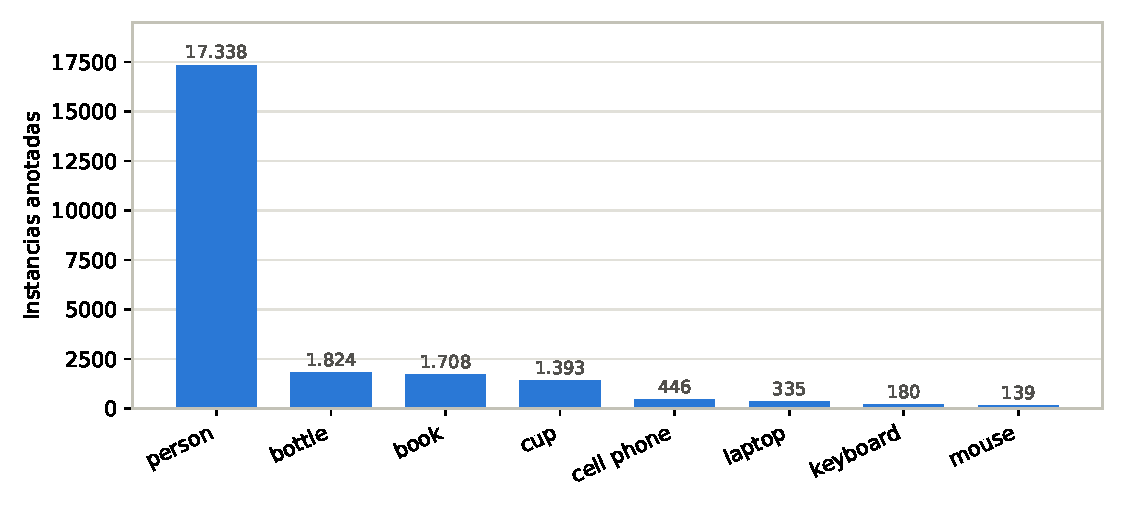
\includegraphics[width=0.85\textwidth]{dist_clases.pdf}
  \caption{Distribución de instancias anotadas por clase en el subconjunto
  construido (5.000 imágenes de COCO 2017).}
  \label{fig:dist}
\end{figure}

\subsection{Particiones}

El subconjunto se dividió en tres particiones disjuntas a nivel de imagen,
con semilla fija: \textbf{entrenamiento} (60\,\%, 3.000 imágenes), destinada
al ajuste de los pesos; \textbf{validación} (15\,\%, 750 imágenes), empleada
para el monitoreo del entrenamiento y la selección del mejor punto de
control; y \textbf{prueba} (25\,\%, 1.250 imágenes), reservada exclusivamente
para la evaluación final, de modo que las métricas reportadas sobre ella no
intervienen en ninguna decisión de entrenamiento. Se verificó que la
distribución de clases se mantuviera aproximadamente proporcional entre
particiones. El Código~\ref{lst:split} implementa la partición.

\begin{lstlisting}[style=py,caption={Partición reproducible 60/15/25\,\% a
nivel de imagen, con control de integridad (particiones disjuntas y
exhaustivas).},label={lst:split}]
# Se quita la etiqueta de split de origen para evitar fuga de datos
dataset.untag_samples(['train', 'validation', 'test'])
four.random_split(view, SPLITS, seed=SEED)   # 60 / 15 / 25 %

# Control: las tres particiones deben cubrir el total sin solaparse
assert sum(view.match_tags(s).count() for s in SPLITS) == view.count()
\end{lstlisting}

\subsection{Conversión al formato YOLO de segmentación}

El entrenador de Ultralytics requiere las anotaciones en formato YOLO de
segmentación: un archivo de texto por imagen en el que cada línea describe una
instancia como un índice de clase seguido de los vértices de su polígono,
normalizados al rango $[0,1]$. La conversión comprendió dos pasos:

\begin{enumerate}
  \item \textbf{De máscaras a polígonos.} Las instancias de COCO cargadas por
  FiftyOne se representan como máscaras binarias; se convirtieron a polígonos
  con una tolerancia de simplificación de 2~píxeles, que reduce el número de
  vértices sin pérdida perceptible de fidelidad geométrica.
  \item \textbf{Saneamiento de fragmentos degenerados.} Las máscaras
  multi-parte (objetos divididos por oclusión) y los objetos muy pequeños
  pueden producir, tras la simplificación, polígonos de menos de tres
  vértices, que el cargador de Ultralytics interpreta como cajas y rechaza.
  Estas líneas ---aproximadamente el 4\,\% del total, fragmentos sin área
  significativa--- se eliminaron de los archivos exportados; la componente
  principal de cada objeto conserva su polígono.
\end{enumerate}

El Código~\ref{lst:export} realiza la conversión de máscaras a polígonos y la
exportación en formato YOLO; el Código~\ref{lst:saneamiento}, el saneamiento
de los fragmentos degenerados.

\begin{lstlisting}[style=py,caption={Conversión de máscaras de instancia a
polígonos y exportación de las tres particiones al formato YOLO de
segmentación.},label={lst:export}]
# Máscaras binarias -> polígonos (tolerancia de simplificación: 2 px)
foul.instances_to_polylines(view, 'ground_truth', 'polylines', tolerance=2)

for split in SPLITS:
    view.match_tags(split).export(
        export_dir=str(DATA_DIR),
        dataset_type=fo.types.YOLOv5Dataset,
        label_field='polylines', split=split, classes=CLASSES,
    )
\end{lstlisting}

\begin{lstlisting}[style=py,caption={Saneamiento: se descartan las líneas cuyo
polígono quedó con menos de tres vértices (que Ultralytics rechazaría).},
label={lst:saneamiento}]
for lbl in (ROOT / 'data').glob('coco_subset*/labels/*/*.txt'):
    lineas = lbl.read_text().strip().splitlines()
    validas = [l for l in lineas if len(l.split()) >= 7]  # clase + >=3 vértices
    if len(validas) != len(lineas):
        lbl.write_text('\n'.join(validas) + '\n' if validas else '')
\end{lstlisting}

Como control de calidad se reconstruyeron las anotaciones a partir de los
archivos exportados y se superpusieron sobre las imágenes correspondientes
(Figura~\ref{fig:verificacion}), validando la cadena completa de conversión:
formato, normalización de coordenadas y asignación de índices de clase.

\begin{figure}[H]
  \centering
  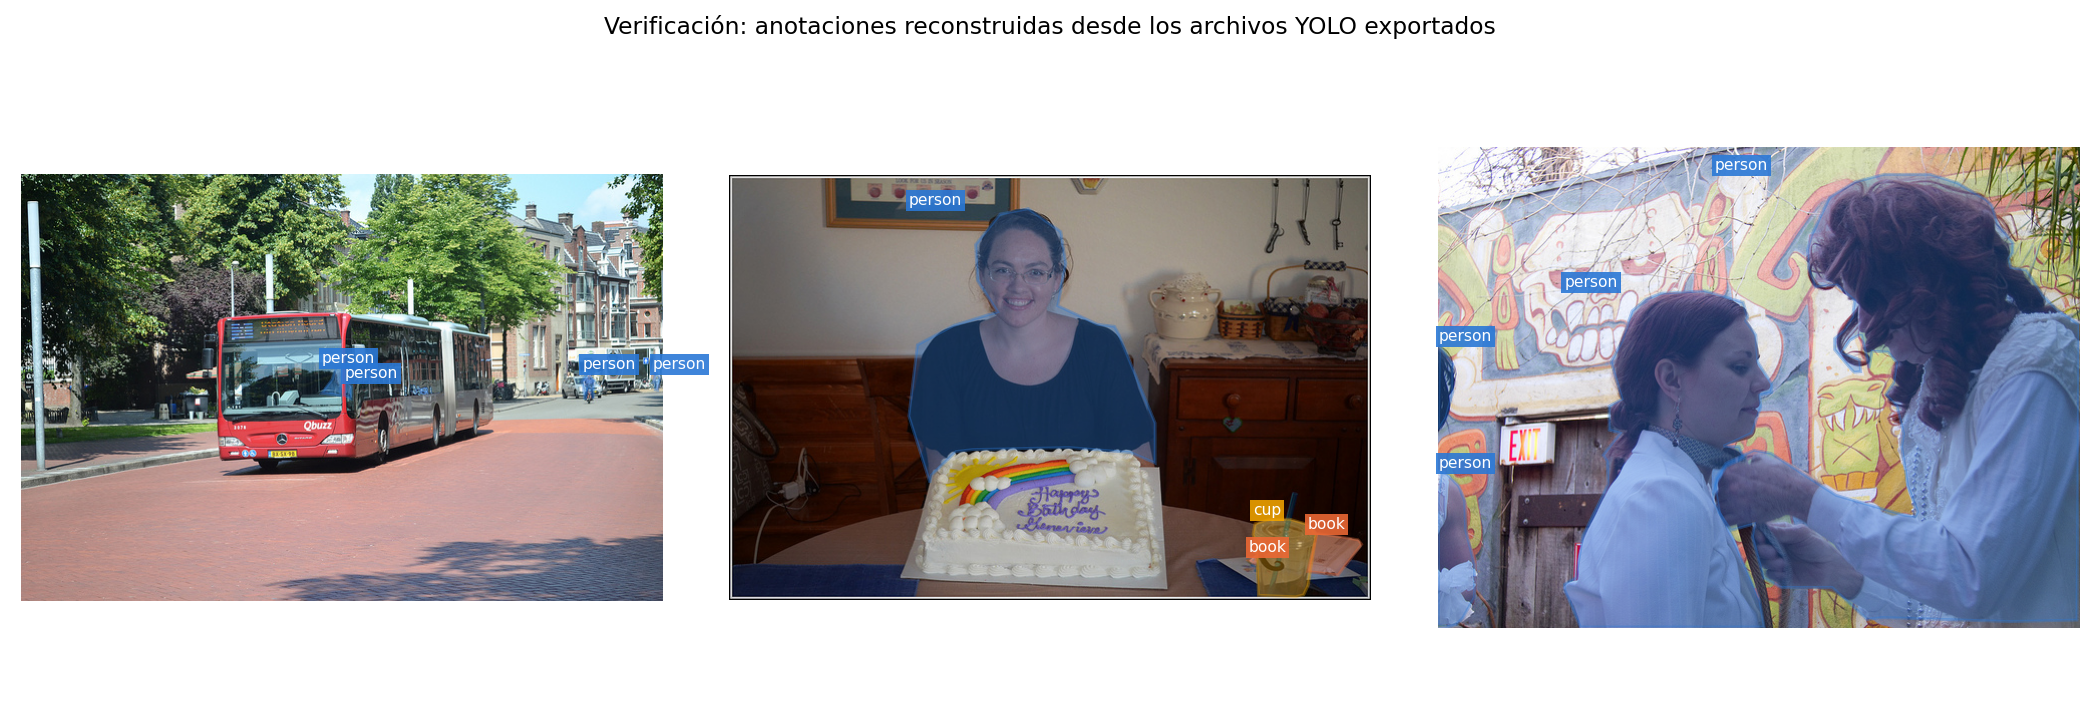
\includegraphics[width=\textwidth]{verificacion_etiquetas.png}
  \caption{Verificación de la conversión: anotaciones reconstruidas desde los
  archivos YOLO exportados, superpuestas sobre tres imágenes de
  entrenamiento. Los polígonos coinciden con los contornos de los objetos y
  las etiquetas de clase son correctas.}
  \label{fig:verificacion}
\end{figure}

% ============================================================================
\section{Metodología}
\label{sec:metodo}

\subsection{Arquitectura: YOLOv8n-seg}

Se adoptó \textbf{YOLOv8-seg} \cite{jocher2023yolov8}, un modelo de
segmentación de instancias de una sola etapa (\emph{one-stage}) y libre de
anclas (\emph{anchor-free}), heredero de la familia YOLO
\cite{redmon2016yolo}. Su arquitectura se compone de:

\begin{itemize}
  \item un \textbf{backbone} convolucional (CSPDarknet con bloques C2f) que
  extrae mapas de características a múltiples escalas;
  \item un \textbf{neck} de tipo PAN-FPN que fusiona información semántica de
  alto nivel con detalle espacial de bajo nivel;
  \item una \textbf{cabeza desacoplada} que predice, para cada objeto, la caja
  delimitadora, la clase y un vector de coeficientes de máscara, junto con una
  rama que genera \emph{prototipos} de máscara a resolución de imagen (esquema
  derivado de YOLACT \cite{bolya2019yolact}). La máscara final de cada
  instancia se obtiene como combinación lineal de los prototipos, lo que
  permite segmentar con costo computacional casi constante por imagen.
\end{itemize}

Se eligió la variante \textbf{nano} (3,26~millones de parámetros,
11,4~GFLOPs), la de menor capacidad de la familia, porque el requisito de
tiempo real debe satisfacerse sobre la CPU de una computadora personal: es la
variante con mejor relación desempeño--latencia para ese escenario.

\textbf{Estrategia de transferencia.} Se partió de los pesos preentrenados en
COCO completo. Al reducir el vocabulario de 80 a 8 clases, el entrenador de
Ultralytics \emph{reinicializa} la rama de clasificación de la cabeza ---cuyas
dimensiones dependen del número de clases--- mientras transfiere el resto de los
pesos: en el registro de entrenamiento, \texttt{Transferred 381/417 items}, con
36 tensores ($\sim$372.000 parámetros) que arrancan desde cero. El
\emph{backbone} y el \emph{neck}, en cambio, heredan íntegramente las
representaciones aprendidas sobre las 118.000 imágenes de COCO.

Esta reinicialización tiene una consecuencia práctica que se documenta en la
Sección~\ref{sec:ablacion}: un ajuste fino \emph{completo} (sin congelamiento)
del clasificador nuevo sobre solo 3.000 imágenes degrada el desempeño respecto
del modelo preentrenado. Dado que el dominio de origen y el de destino coinciden
---las ocho clases pertenecen a COCO---, la estrategia adoptada es
\textbf{congelar el backbone} (\texttt{freeze=10}) para preservar sus
representaciones y concentrar el presupuesto de optimización en el \emph{neck} y
la cabeza, ampliando el número de épocas para que el clasificador reinicializado
alcance a converger.

\subsection{Preprocesamiento y aumento de datos}

\textbf{Preprocesamiento} (entrenamiento e inferencia): toda imagen se
redimensiona a $640\times640$ píxeles mediante \emph{letterbox} (se preserva
la relación de aspecto y se rellena con bordes neutros) y las intensidades se
normalizan al rango $[0,1]$.

\textbf{Aumento de datos} (solo entrenamiento): amplía artificialmente la
variabilidad del conjunto de entrenamiento y actúa como regularizador. Se
empleó el esquema estándar de Ultralytics, que transforma de manera
consistente las imágenes \emph{y} sus polígonos de segmentación. La
Tabla~\ref{tab:aug} resume las transformaciones y su justificación; la
Figura~\ref{fig:mosaico} ilustra un lote de entrenamiento real con
\emph{mosaic}. Se omitieron el volteo vertical, las rotaciones y
\emph{mixup}, que generarían poses inverosímiles para el dominio sin
beneficio esperado.

\begin{table}[H]
  \centering
  \small
  \caption{Esquema de aumento de datos empleado durante el entrenamiento.}
  \label{tab:aug}
  \begin{tabular}{@{}llp{8.2cm}@{}}
    \toprule
    \textbf{Transformación} & \textbf{Valor} & \textbf{Justificación} \\
    \midrule
    \emph{Mosaic} & 1,0 & Compone cuatro imágenes en una: expone al modelo a
    objetos en contextos y escalas atípicos. Se desactiva en las últimas 10
    épocas (\texttt{close\_mosaic}=10). \\
    Volteo horizontal & $p=0,5$ & Los objetos del dominio no tienen
    quiralidad relevante; duplica la variabilidad de pose. \\
    Traslación & $\pm$10\,\% & Robustez ante encuadres imperfectos,
    frecuentes en una cámara web. \\
    Escala & $\pm$50\,\% & Robustez ante variaciones de distancia
    objeto--cámara, críticas para la demostración en vivo. \\
    Perturbación HSV & $h{=}0{,}015$; $s{=}0{,}7$; $v{=}0{,}4$ & Robustez ante
    cambios de iluminación y balance de color entre las escenas de COCO y la
    cámara del usuario. \\
    \bottomrule
  \end{tabular}
\end{table}

\begin{figure}[H]
  \centering
  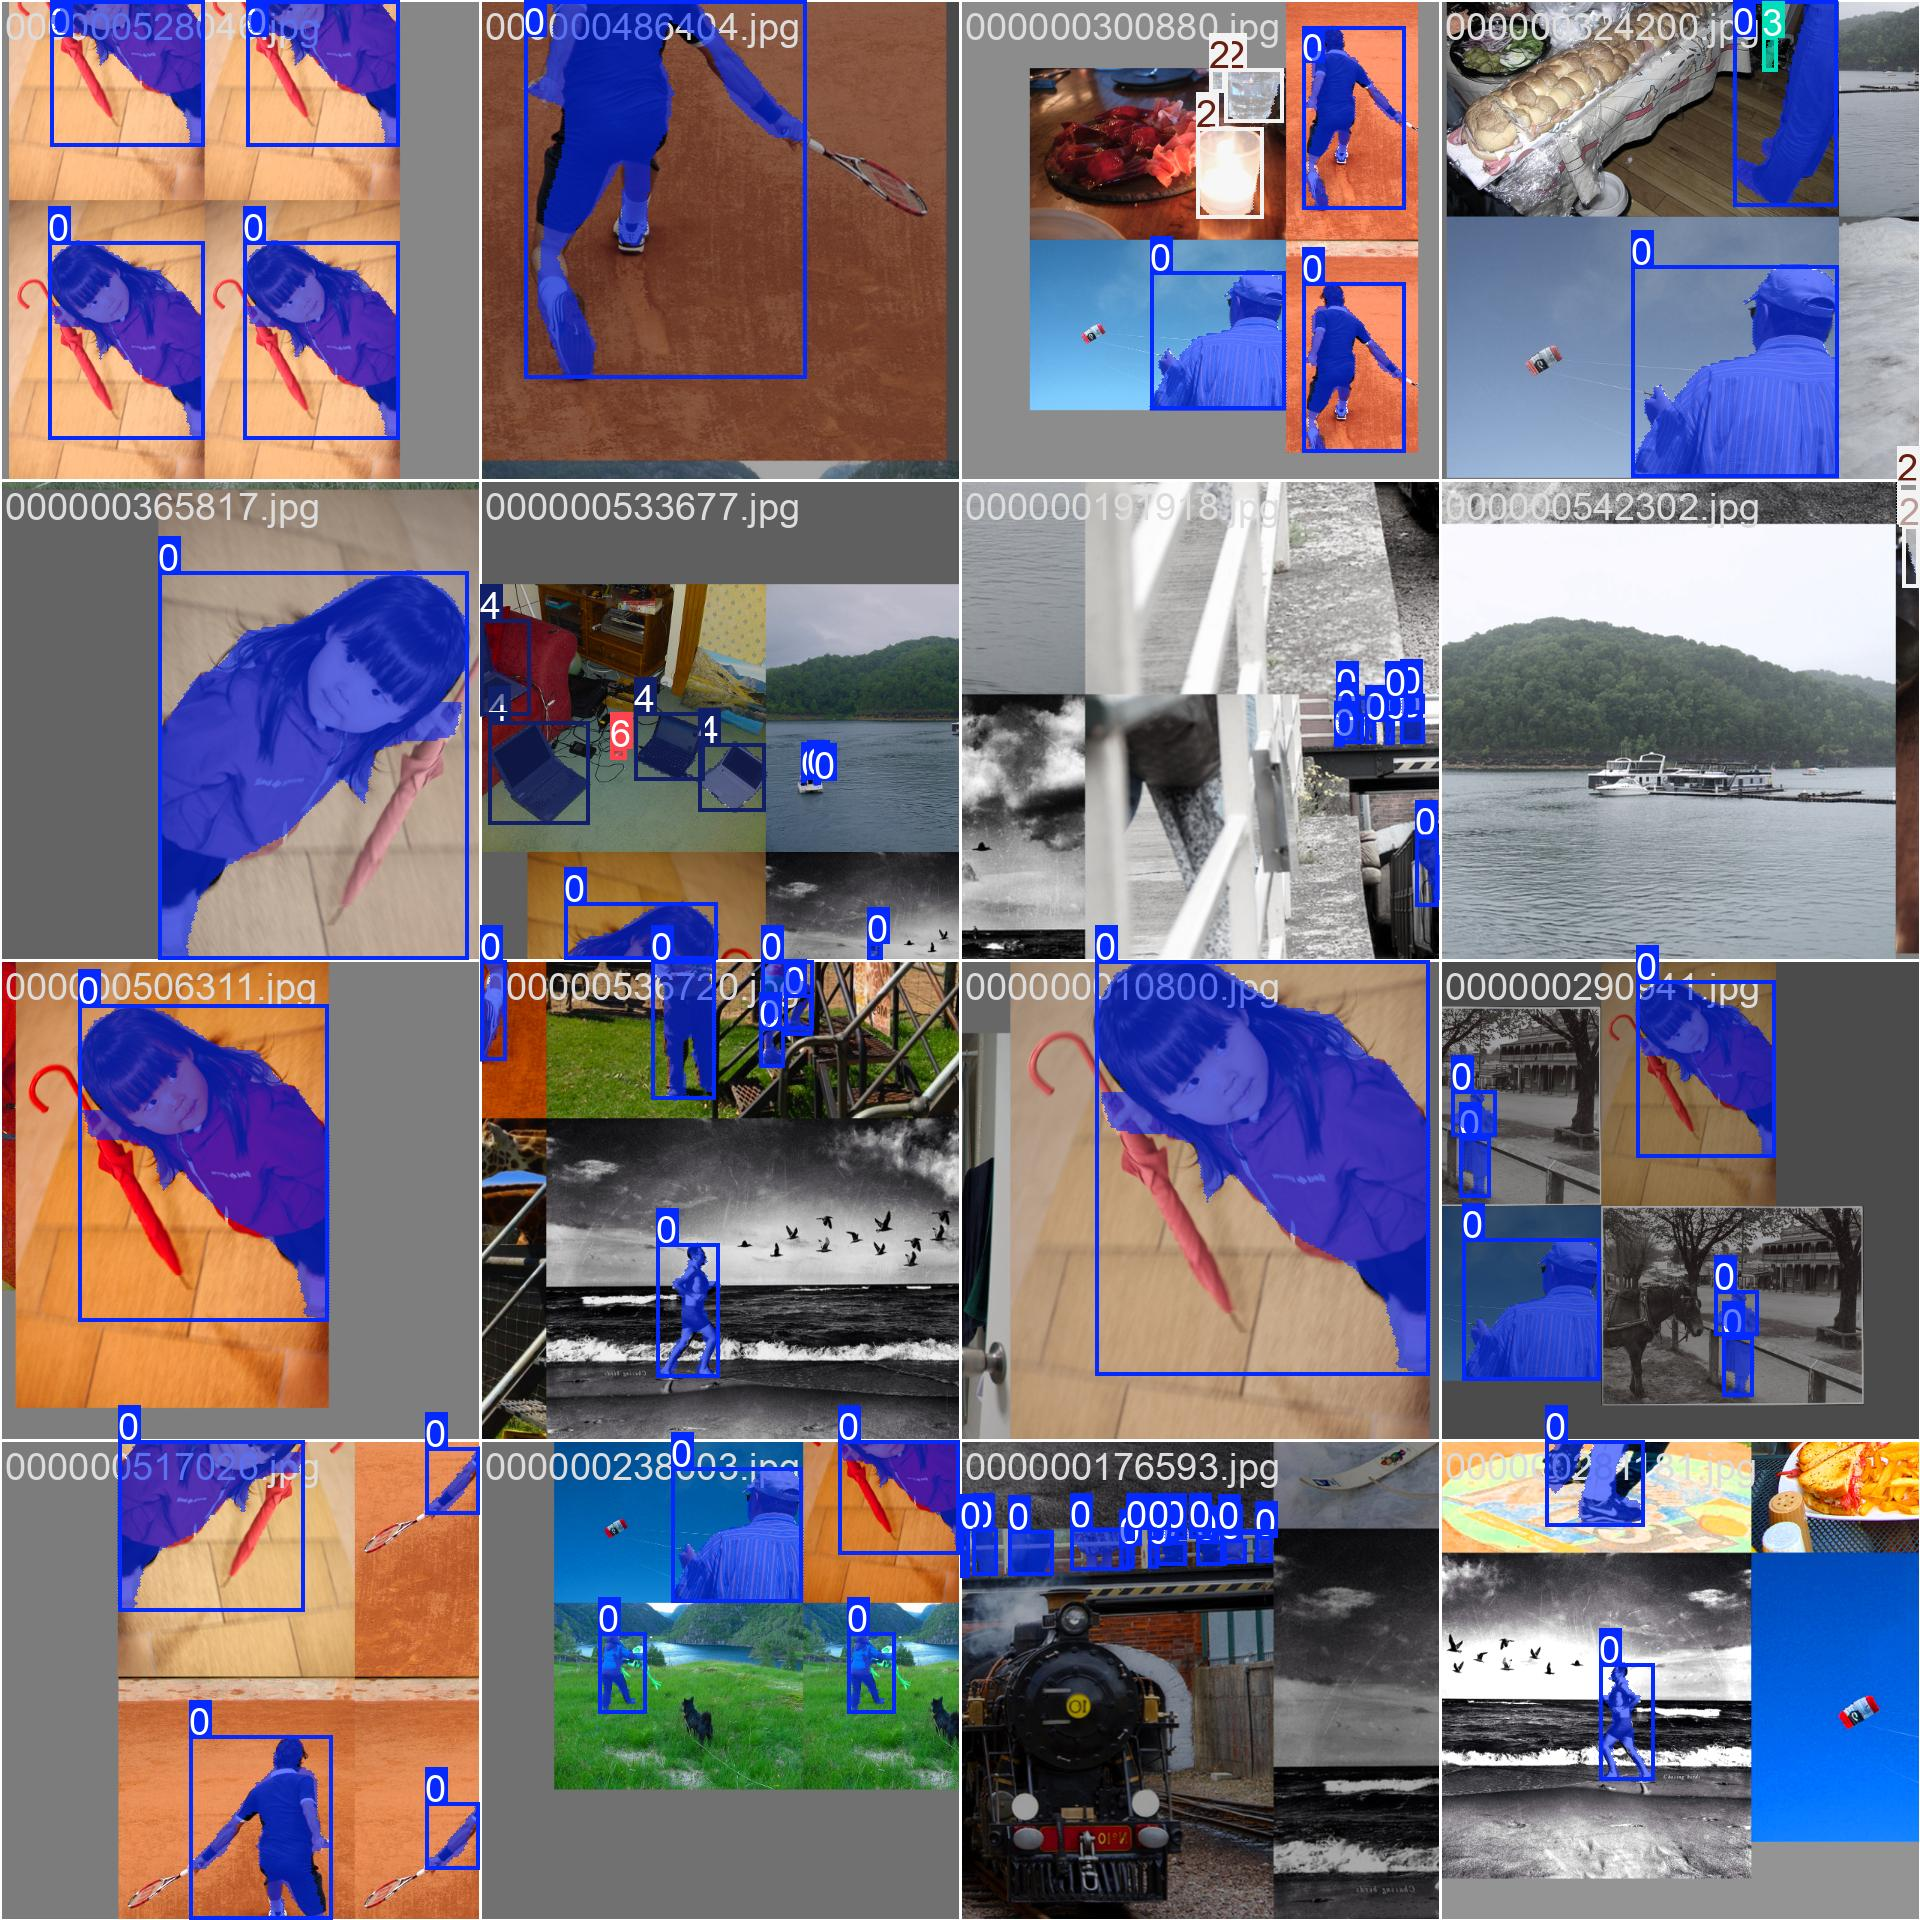
\includegraphics[width=0.8\textwidth]{mosaico_entrenamiento.jpg}
  \caption{Lote de entrenamiento real con aumento \emph{mosaic}: cada muestra
  compone cuatro imágenes con sus máscaras transformadas de manera
  consistente.}
  \label{fig:mosaico}
\end{figure}

Estas transformaciones se declararon de forma explícita
(Código~\ref{lst:aug}) para documentar la configuración y pasarlas al
entrenador.

\begin{lstlisting}[style=py,caption={Hiperparámetros de aumento de datos,
declarados explícitamente y pasados luego a \texttt{model.train}.},
label={lst:aug}]
AUG = dict(
    mosaic=1.0, close_mosaic=10,           # mosaic, desactivado en las últimas 10 épocas
    fliplr=0.5, flipud=0.0,                # solo volteo horizontal
    degrees=0.0, translate=0.1, scale=0.5, shear=0.0,
    hsv_h=0.015, hsv_s=0.7, hsv_v=0.4,     # perturbación de color/iluminación
    mixup=0.0,
)
\end{lstlisting}

\subsection{Configuración del entrenamiento}
\label{sec:config}

El entrenamiento se ejecutó en un servidor con GPU NVIDIA GeForce RTX~5090
(32~GB), con Ultralytics~8.4.89, PyTorch~2.12.1 (CUDA~13.0) y Python~3.12. La
Tabla~\ref{tab:config} resume la configuración. El tamaño de lote se fijó
explícitamente en 32 y los procesos de precarga de datos en 4, valores
elegidos para acotar el consumo de memoria del sistema en el servidor
compartido. El optimizador AdamW \cite{loshchilov2019adamw} y su tasa de
aprendizaje fueron seleccionados por la heurística automática de Ultralytics.
El entrenamiento, previsto para 150 épocas, se detuvo por \emph{early stopping}
en la época~140 (sin mejora durante 50 épocas); el mejor punto de control se
seleccionó por la métrica de aptitud de Ultralytics sobre la partición de
validación.

\begin{table}[H]
  \centering
  \small
  \caption{Configuración del entrenamiento.}
  \label{tab:config}
  \begin{tabular}{@{}ll@{}}
    \toprule
    \textbf{Parámetro} & \textbf{Valor} \\
    \midrule
    Modelo base & \texttt{yolov8n-seg.pt} (preentrenado en COCO) \\
    Capas congeladas & \texttt{freeze=10} (\emph{backbone}); se entrenan \emph{neck} y cabeza \\
    Épocas & 150 (early stopping con paciencia 50; se detuvo en la 140) \\
    Resolución de entrada & $640\times640$ (letterbox) \\
    Tamaño de lote & 32 \\
    Optimizador & AdamW (selección automática), $lr_0 = 8{,}33\times10^{-4}$,
    momento 0,9 \\
    Decaimiento de pesos & $5\times10^{-4}$ \\
    Precisión mixta (AMP) & Sí \\
    Semilla & 42 (modo determinista) \\
    Duración total & 132 minutos \\
    \bottomrule
  \end{tabular}
\end{table}

El ajuste fino se lanza a partir de los pesos preentrenados con una única
llamada al entrenador de Ultralytics (Código~\ref{lst:train}).

\begin{lstlisting}[style=py,caption={Ajuste fino de YOLOv8n-seg desde los pesos
preentrenados en COCO, con el \emph{backbone} congelado y los hiperparámetros de
aumento del Código~\ref{lst:aug}.},label={lst:train}]
model = YOLO('yolov8n-seg.pt')          # pesos preentrenados en COCO (80 clases)

resultados = model.train(
    data=str(DATA_YAML), epochs=150, imgsz=640,
    batch=32, workers=4,                # acotan el consumo de memoria
    device=0, seed=SEED,
    freeze=10,                          # congela el backbone (capas 0-9)
    patience=50,                        # early stopping
    project=str(RUNS_DIR), name='yolov8n_seg_tpf',
    **AUG,
)
\end{lstlisting}

% ============================================================================
\section{Experimentos y resultados}
\label{sec:resultados}

\subsection{Protocolo de evaluación}

Las métricas siguen el protocolo estándar de COCO. El \textbf{IoU}
(\emph{Intersection over Union}) mide el solapamiento entre una predicción
$P$ y su anotación de referencia $G$:
\begin{equation}
  IoU(P, G) = \frac{|P \cap G|}{|P \cup G|},
\end{equation}
y se aplica tanto a cajas delimitadoras como a máscaras. Una predicción es un
verdadero positivo si su IoU con una anotación de la misma clase supera un
umbral dado. La \textbf{AP} (\emph{Average Precision}) de una clase es el
área bajo su curva precisión--recall, y el \textbf{mAP} es su promedio sobre
las clases. Se reportan las dos variantes estándar: \textbf{mAP@50} (umbral
de IoU de 0,5, criterio laxo) y \textbf{mAP@50-95} (promedio sobre umbrales
de 0,5 a 0,95 en pasos de 0,05, criterio estricto que premia la precisión de
la localización), calculadas por separado para cajas (detección) y máscaras
(segmentación). Toda la evaluación de esta sección se realiza sobre la
partición de \textbf{prueba} (1.250 imágenes, 7.117 instancias), invocando al
evaluador de Ultralytics sobre el \emph{split} de prueba (Código~\ref{lst:val}).

\begin{lstlisting}[style=py,caption={Evaluación del modelo ajustado sobre la
partición de prueba; \texttt{plots=True} genera la matriz de confusión y las
curvas precisión--recall.},label={lst:val}]
metrics = model.val(
    data=str(DATA_DIR / 'dataset.yaml'),
    split='test',          # partición de prueba reservada
    plots=True,
)
\end{lstlisting}

\subsection{Curvas de aprendizaje}

La Figura~\ref{fig:curvas} muestra la evolución del entrenamiento. Las
pérdidas de caja y de segmentación decrecen de forma sostenida tanto en
entrenamiento como en validación, sin divergencia entre ambas ---no se
observa sobreajuste. La pérdida de validación se ubica levemente por
\emph{encima} de la de entrenamiento, como corresponde a la brecha de
generalización habitual sobre una partición genuinamente reservada. El mAP de
validación crece con rapidez en las primeras $\sim$20 épocas y luego se
estabiliza en una meseta (mAP@50 de cajas: de 0,26 en la primera época a
$\sim$0,47; mAP@50-95 de máscaras hasta 0,283), coherente con un modelo cuyo
\emph{backbone} está congelado y cuya capacidad de ajuste se concentra en el
\emph{neck} y la cabeza. El \emph{early stopping} detuvo el entrenamiento en la
época~140, 50 épocas después del mejor punto de control (época~90).

\begin{figure}[H]
  \centering
  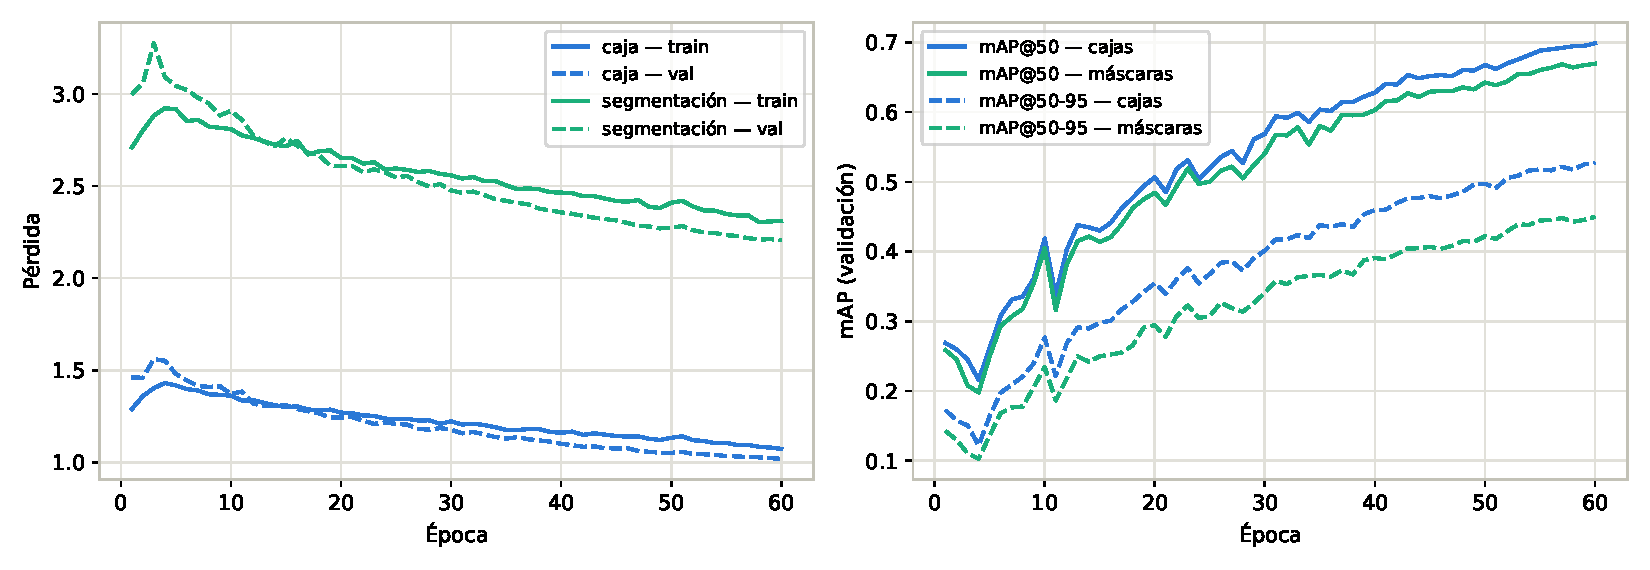
\includegraphics[width=\textwidth]{curvas_entrenamiento.pdf}
  \caption{Evolución del entrenamiento. Izquierda: pérdidas de caja y de
  segmentación en entrenamiento (línea continua) y validación (línea
  discontinua). Derecha: mAP@50 y mAP@50-95 sobre la partición de validación,
  para cajas y máscaras.}
  \label{fig:curvas}
\end{figure}

\subsection{Métricas sobre la partición de prueba}

La Tabla~\ref{tab:global} resume las métricas globales del modelo ajustado
sobre la partición de prueba y la Tabla~\ref{tab:porclase} las desglosa por
clase; la Figura~\ref{fig:porclase} las presenta gráficamente.

\begin{table}[H]
  \centering
  \small
  \caption{Métricas globales sobre la partición de prueba (1.250 imágenes,
  7.117 instancias).}
  \label{tab:global}
  \begin{tabular}{@{}lcc@{}}
    \toprule
    \textbf{Métrica} & \textbf{Cajas (detección)} & \textbf{Máscaras (segmentación)} \\
    \midrule
    Precisión media & 0,577 & 0,559 \\
    Recall medio    & 0,397 & 0,383 \\
    mAP@50          & 0,440 & 0,420 \\
    mAP@50-95       & \textbf{0,292} & \textbf{0,246} \\
    \bottomrule
  \end{tabular}
\end{table}

\begin{table}[H]
  \centering
  \small
  \caption{Métricas por clase sobre la partición de prueba.}
  \label{tab:porclase}
  \begin{tabular}{@{}lrcccc@{}}
    \toprule
    & & \multicolumn{2}{c}{\textbf{Cajas}} & \multicolumn{2}{c}{\textbf{Máscaras}} \\
    \cmidrule(lr){3-4}\cmidrule(lr){5-6}
    \textbf{Clase} & \textbf{Instancias} & \textbf{mAP@50} & \textbf{mAP@50-95}
    & \textbf{mAP@50} & \textbf{mAP@50-95} \\
    \midrule
    person     & 5.448 & 0,596 & 0,378 & 0,572 & 0,316 \\
    cell phone &   103 & 0,194 & 0,113 & 0,185 & 0,099 \\
    cup        &   415 & 0,426 & 0,273 & 0,416 & 0,262 \\
    bottle     &   527 & 0,423 & 0,260 & 0,405 & 0,216 \\
    laptop     &    94 & 0,736 & 0,554 & 0,715 & 0,437 \\
    keyboard   &    40 & 0,337 & 0,198 & 0,301 & 0,163 \\
    mouse      &    35 & 0,686 & 0,512 & 0,685 & 0,447 \\
    book       &   455 & 0,119 & 0,051 & 0,077 & 0,025 \\
    \midrule
    \textbf{Todas} & 7.117 & 0,440 & 0,292 & 0,420 & 0,246 \\
    \bottomrule
  \end{tabular}
\end{table}

\begin{figure}[H]
  \centering
  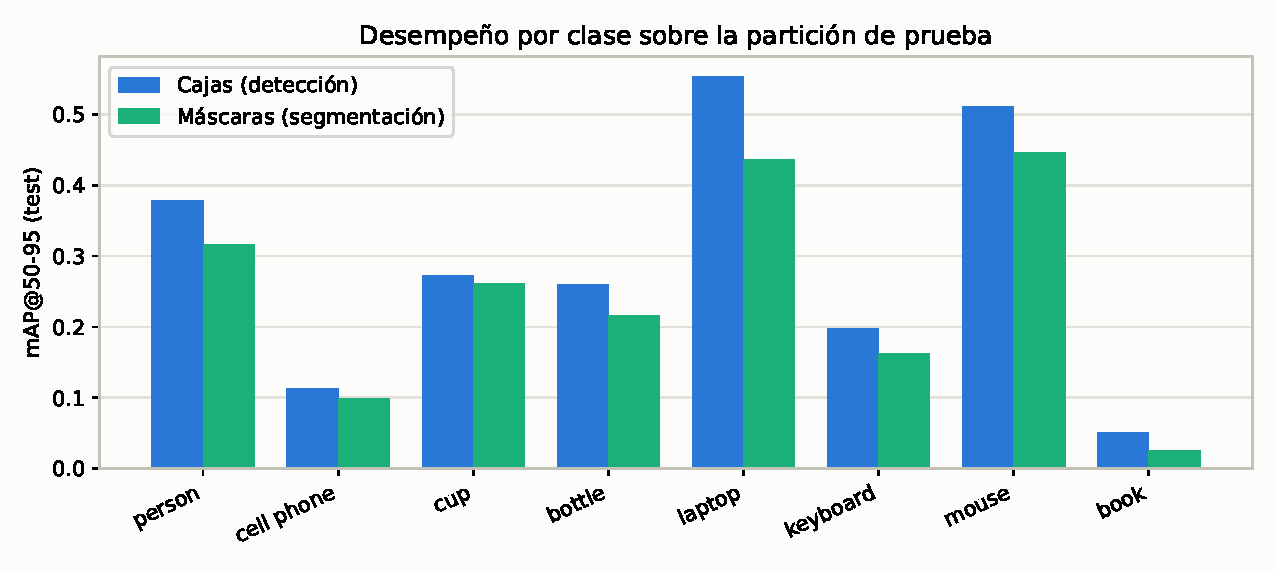
\includegraphics[width=0.85\textwidth]{map_por_clase.pdf}
  \caption{mAP@50-95 por clase sobre la partición de prueba, para cajas y
  máscaras.}
  \label{fig:porclase}
\end{figure}

Del desglose surgen tres observaciones:

\begin{itemize}
  \item \textbf{Mejores clases: laptop y mouse} (mAP@50-95 de cajas de 0,554 y
  0,512). Son objetos rígidos, de contorno regular y que suelen aparecer a
  escala considerable y poco ocluidos, condiciones favorables tanto para la
  localización como para la segmentación.
  \item \textbf{Peor clase: book} (0,051 en cajas, 0,025 en máscaras). En
  COCO los libros aparecen mayoritariamente apilados o en estanterías, en
  instancias pequeñas, parcialmente visibles y con límites ambiguos entre
  ejemplares contiguos; la propia anotación de referencia es inconsistente en
  esos casos. Es una dificultad conocida de esta categoría.
  \item \textbf{El desempeño global es modesto y está limitado por el recall}
  (0,397 en cajas), no por la precisión (0,577): el modelo acierta cuando
  detecta, pero omite muchas instancias. La Sección~\ref{sec:baseline}
  contextualiza estos valores frente al modelo preentrenado bajo una comparación
  imparcial, y el análisis de la matriz de confusión confirma que el modo de
  error dominante es la omisión.
  \item \textbf{Las máscaras puntúan sistemáticamente por debajo de las
  cajas} (0,246 frente a 0,292 global). El criterio de IoU a nivel de píxel
  es más estricto que el de solapamiento de rectángulos, en particular para
  contornos complejos como los de \texttt{person}, donde la diferencia es
  máxima (0,316 frente a 0,378).
\end{itemize}

\subsection{Matriz de confusión y curvas precisión--recall}

La matriz de confusión normalizada (Figura~\ref{fig:confusion}) muestra que el
modelo prácticamente \textbf{no confunde clases entre sí}: la mayor confusión
inter-clase es de apenas 0,03 (\texttt{cup} con \texttt{bottle}). El modo de
error dominante ---y marcadamente severo--- es la \textbf{omisión} (objetos
reales clasificados como fondo), que afecta sobre todo a \texttt{book} (88\,\%
de sus instancias), \texttt{cell phone} (75\,\%), \texttt{keyboard} (55\,\%),
\texttt{cup} (54\,\%) y \texttt{bottle} (53\,\%), y en menor medida a
\texttt{laptop} (24\,\%). Este patrón es coherente con el análisis por clase:
el vocabulario reducido hace que el problema de clasificación sea sencillo, y
el desafío restante ---el que gobierna el mAP--- es el \textbf{recall} sobre
instancias pequeñas u ocluidas. Las curvas precisión--recall
(Figura~\ref{fig:pr}) muestran el mismo ordenamiento de clases en ambas tareas.

\begin{figure}[H]
  \centering
  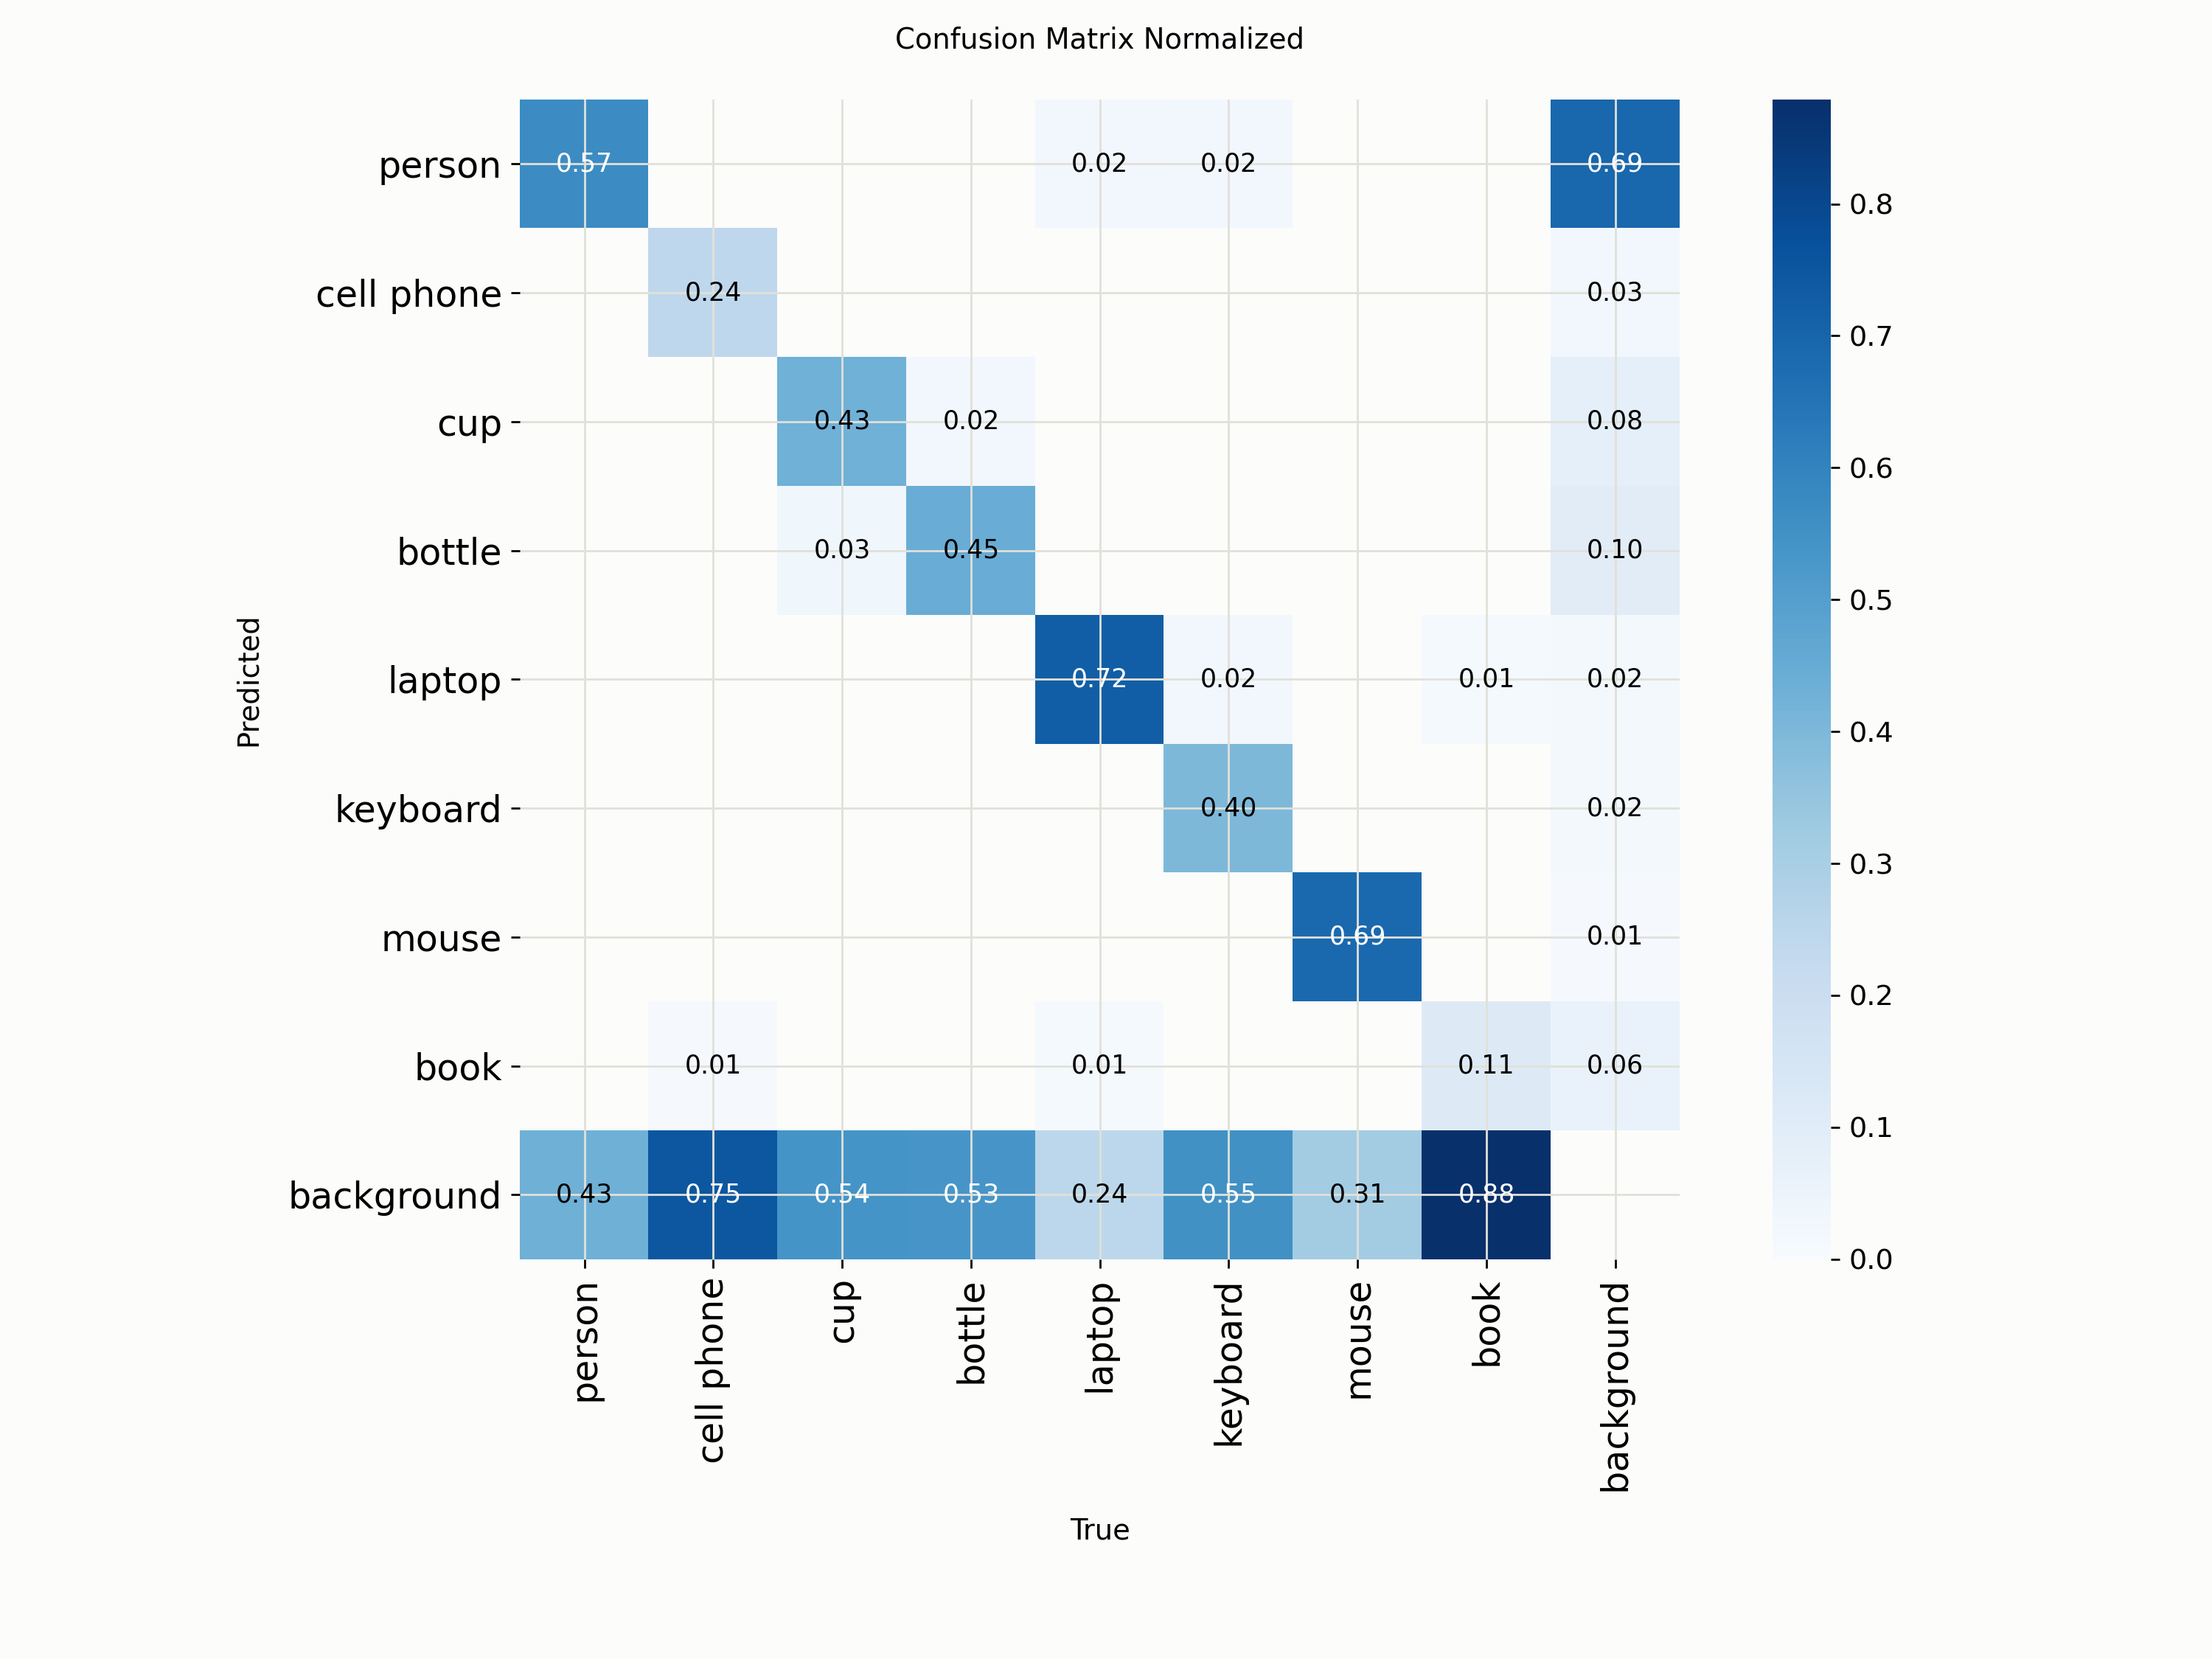
\includegraphics[width=0.8\textwidth]{confusion_matrix.png}
  \caption{Matriz de confusión normalizada por columnas sobre la partición de
  prueba (columnas: clase real; filas: clase predicha). La diagonal concentra
  las predicciones correctas; la última fila corresponde a objetos reales no
  detectados (omisiones).}
  \label{fig:confusion}
\end{figure}

\begin{figure}[H]
  \centering
  \begin{subfigure}[b]{0.49\textwidth}
    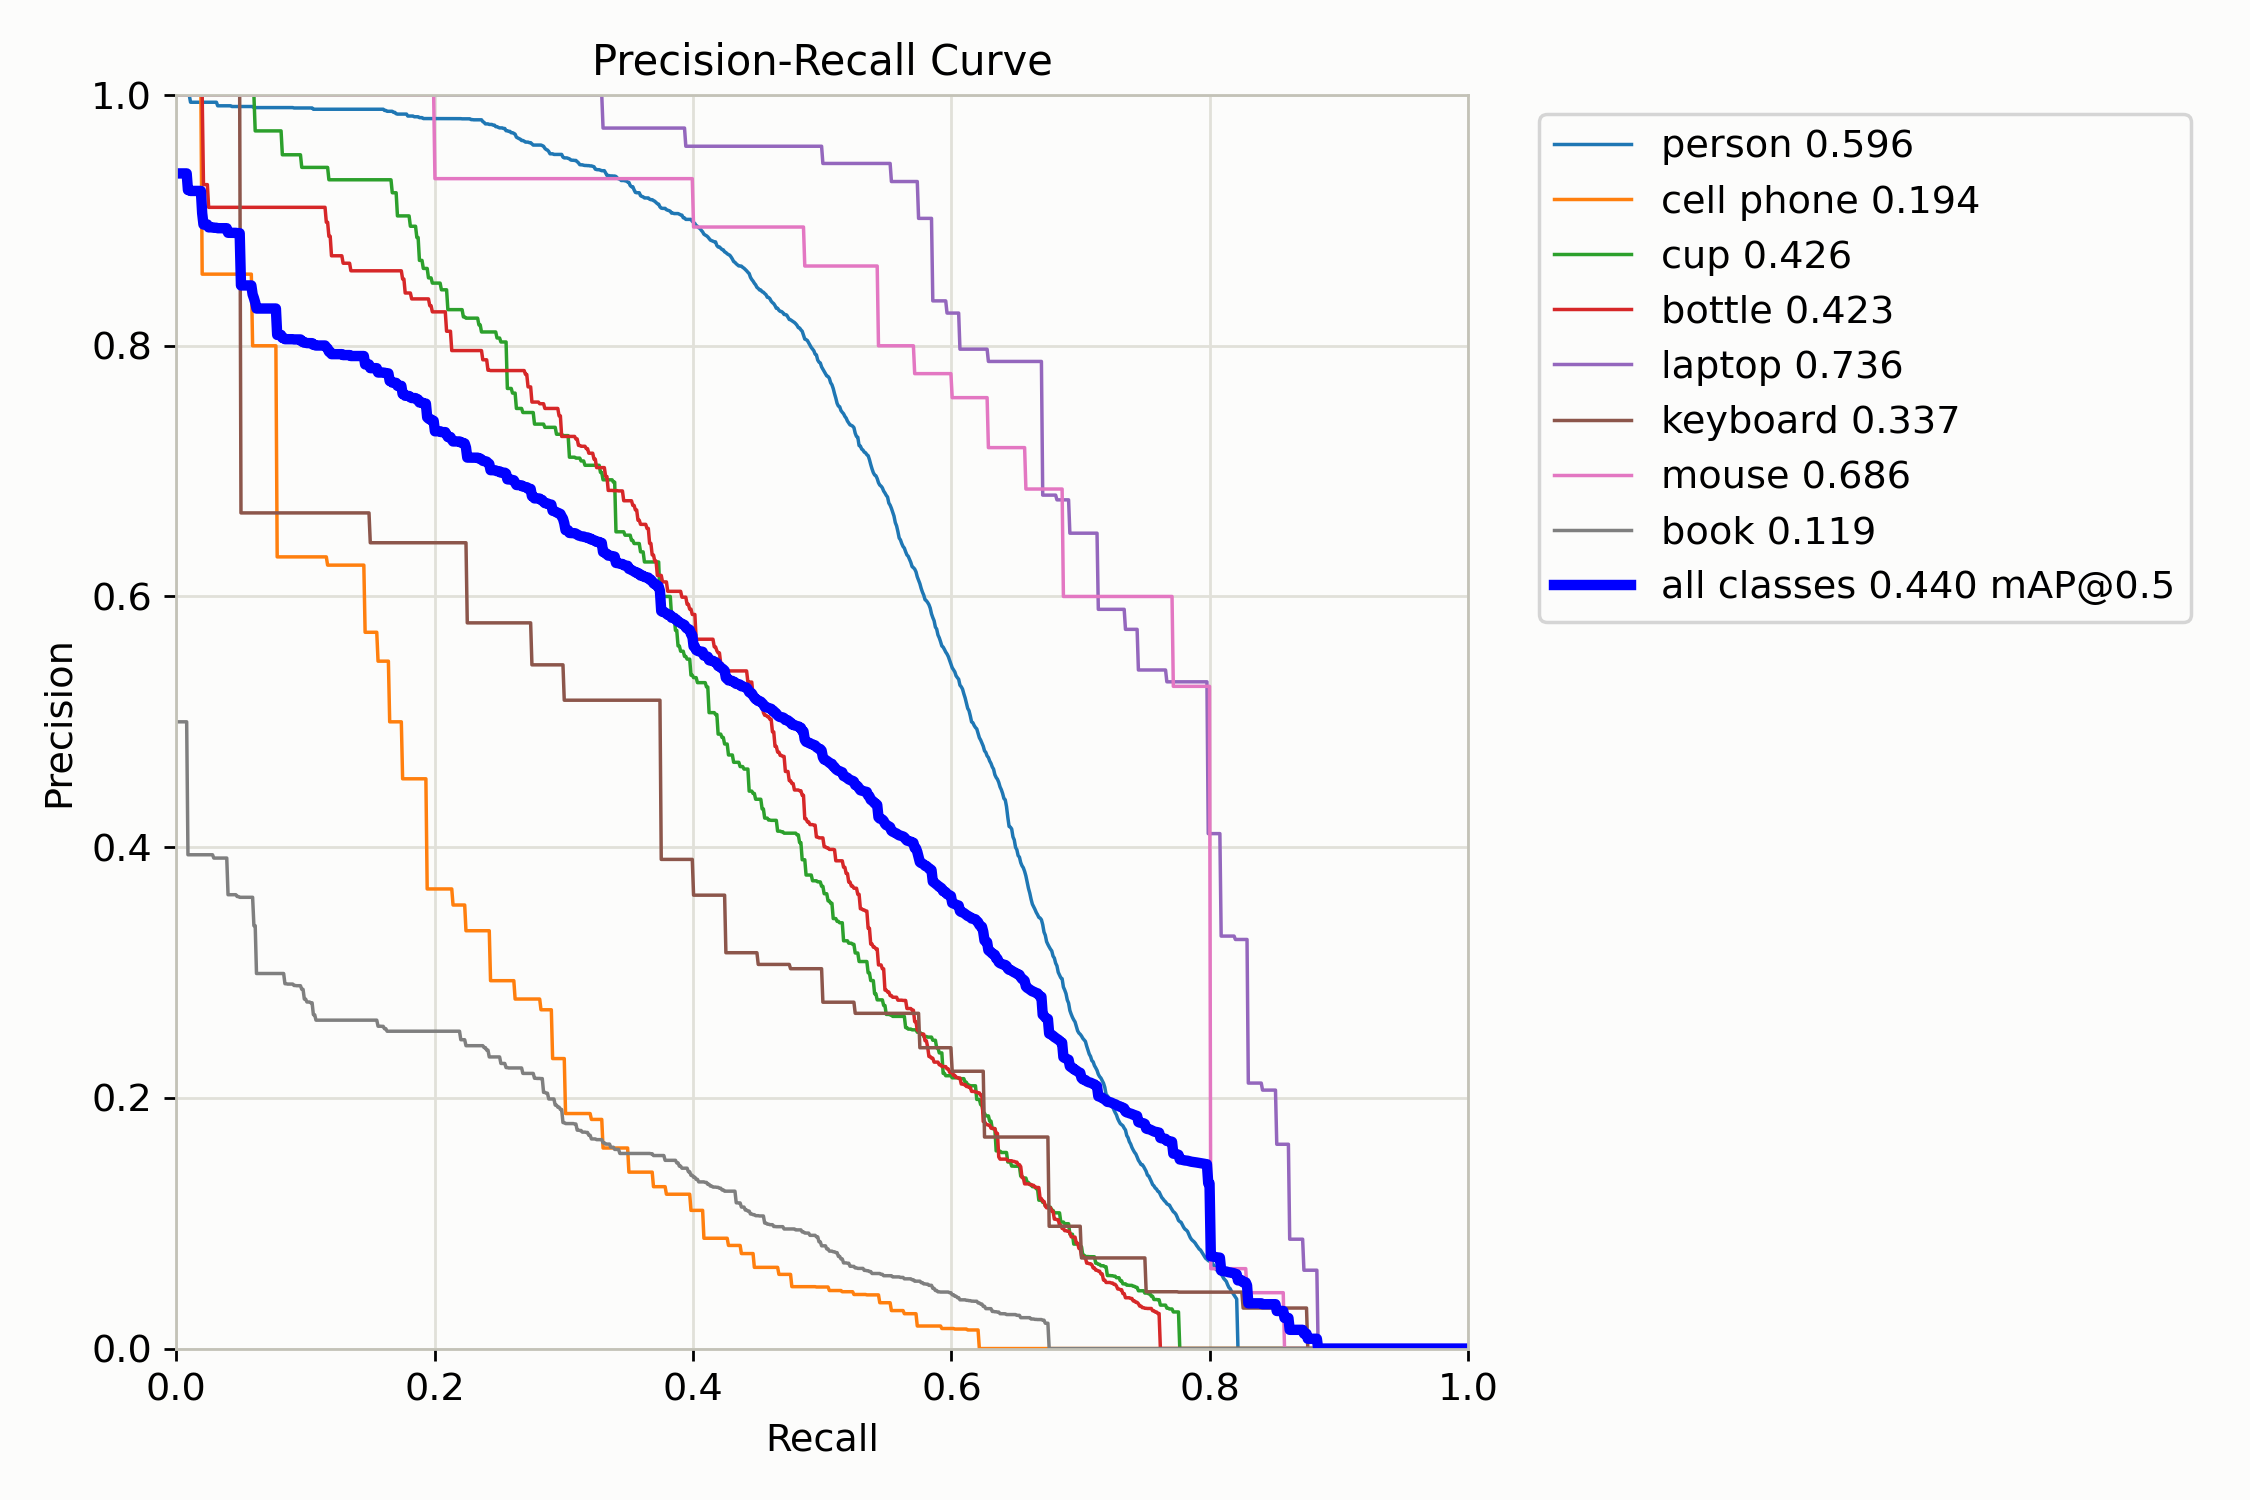
\includegraphics[width=\textwidth]{pr_box.png}
    \caption{Cajas (detección).}
  \end{subfigure}
  \hfill
  \begin{subfigure}[b]{0.49\textwidth}
    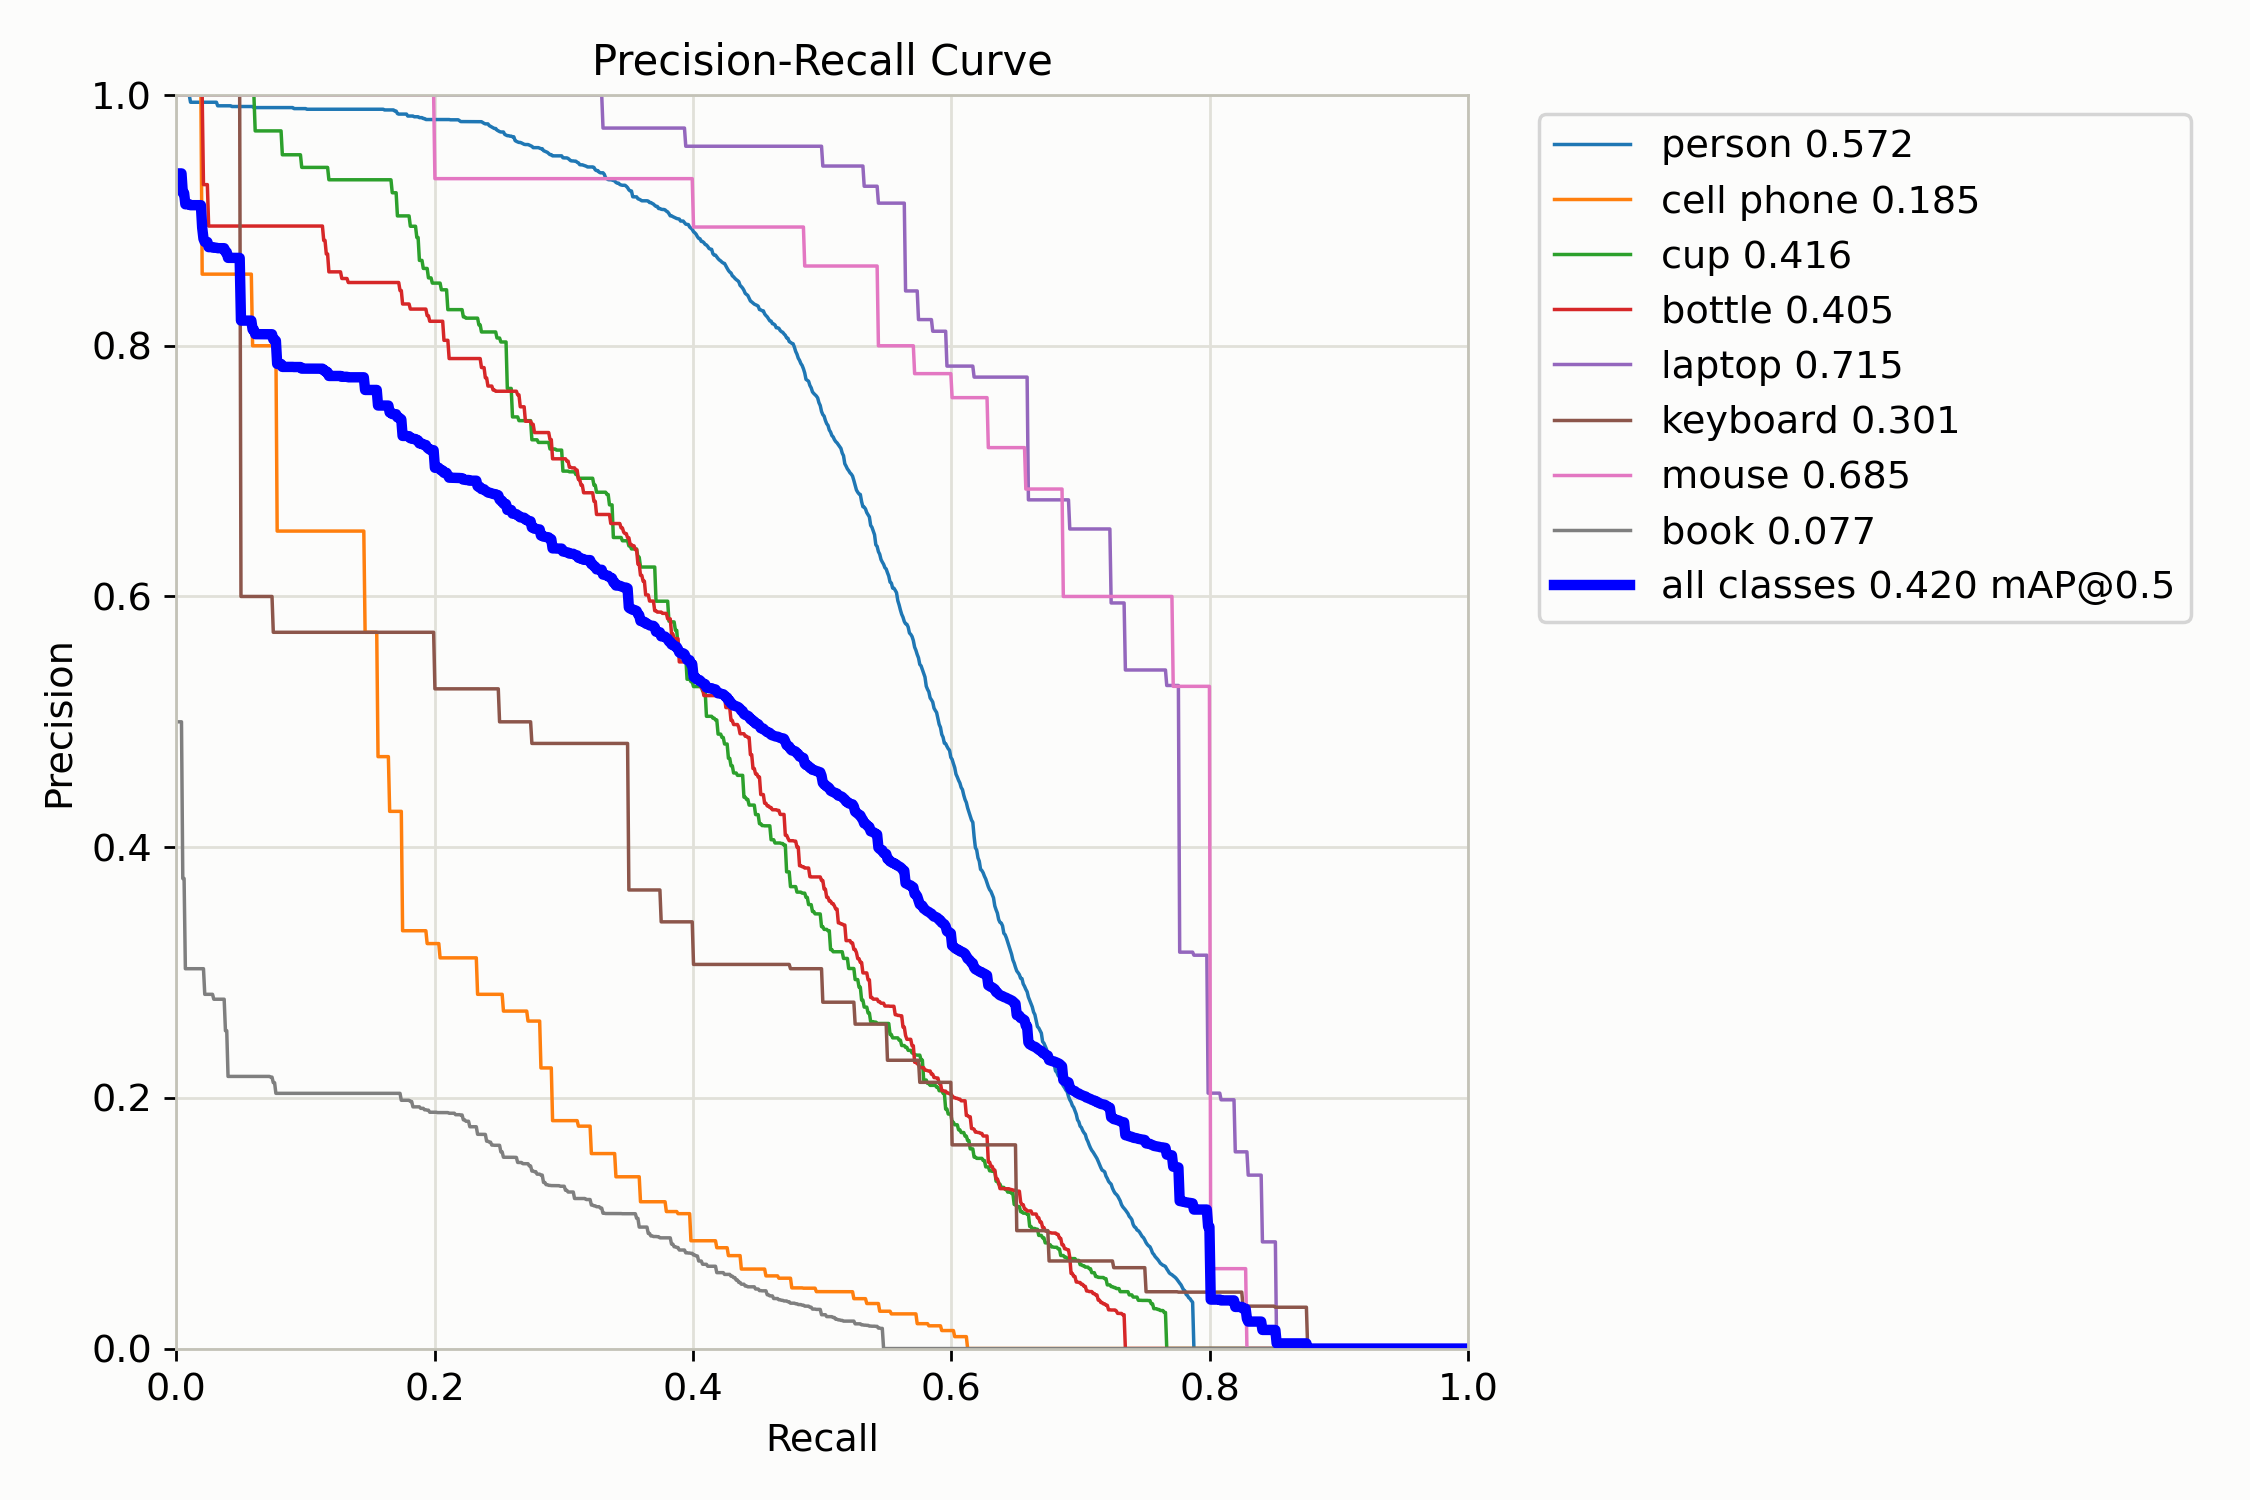
\includegraphics[width=\textwidth]{pr_mask.png}
    \caption{Máscaras (segmentación).}
  \end{subfigure}
  \caption{Curvas precisión--recall por clase sobre la partición de prueba,
  con umbral de IoU de 0,5. El área bajo cada curva es la AP@50 de la clase.}
  \label{fig:pr}
\end{figure}

\subsection{Comparación imparcial con el modelo de referencia}
\label{sec:baseline}

Una forma habitual de cuantificar el aporte del ajuste fino es comparar el
modelo ajustado contra el \textbf{preentrenado original}
(\texttt{yolov8n-seg.pt}, 80 clases) sobre la misma partición de prueba.
Evaluado así, el preentrenado alcanza un mAP@50-95 de máscaras de 0,342,
\emph{por encima} del modelo ajustado (0,246). Sin embargo, esta comparación
está \textbf{sesgada a favor del baseline} por una razón sutil pero decisiva:
el modelo preentrenado se entrenó sobre COCO~train2017, el mismo conjunto del
que se muestrearon nuestras 5.000 imágenes. Por lo tanto, el baseline
\emph{ya vio durante su preentrenamiento las imágenes que aquí se usan como
prueba}, mientras que el modelo ajustado se evalúa sobre datos genuinamente
reservados. Comparar a ambos sobre esa partición mide, en parte, la memoria del
baseline sobre sus propios datos de entrenamiento.

Para una comparación equitativa se construyó una \textbf{partición de prueba
independiente a partir de COCO~val2017}: el conjunto de validación oficial de
COCO, que el modelo preentrenado nunca empleó para ajustar sus pesos y que es
disjunto de train2017 ---y, por lo tanto, de nuestro conjunto de entrenamiento.
Sobre esas 1.250 imágenes (7.249 instancias), \emph{ninguno} de los dos modelos
vio los datos durante su entrenamiento, de modo que la comparación es limpia.
Se replicó la cadena de construcción de datos de la Sección~\ref{sec:datos}
sobre val2017 y se evaluó a ambos modelos sobre ella (Código~\ref{lst:baseline}).

\begin{lstlisting}[style=py,caption={Construcción de una partición de prueba
imparcial desde COCO val2017 (no vista por ninguno de los dos modelos) y
evaluación equitativa del ajustado y del preentrenado sobre ella.},
label={lst:baseline}]
# Partición independiente desde COCO val2017 (misma receta que el Notebook 01)
val_fair = foz.load_zoo_dataset('coco-2017', split='validation',
    label_types=['segmentations'], classes=CLASSES, max_samples=1250, seed=SEED)
# ... export en formato YOLO con vocabulario de 8 y de 80 clases ...

# Evaluación equitativa: ambos modelos sobre los MISMOS datos no vistos
m_ft   = YOLO('models/yolov8n_seg_best.pt')          # ajustado (8 clases)
m_base = YOLO('yolov8n-seg.pt')                       # preentrenado (80 clases)
r_ft   = m_ft.val(data=str(FAIR8  / 'dataset.yaml'), split='val')
r_base = m_base.val(data=str(FAIR80 / 'dataset.yaml'), split='val')
\end{lstlisting}

\begin{table}[H]
  \centering
  \small
  \caption{Comparación imparcial del mAP@50-95 de máscaras por clase, sobre la
  partición independiente de COCO val2017 (datos no vistos por ninguno de los
  dos modelos), entre el preentrenado de referencia y el modelo ajustado.}
  \label{tab:baseline}
  \begin{tabular}{@{}lccc@{}}
    \toprule
    \textbf{Clase} & \textbf{Baseline preentrenado} & \textbf{Ajustado (este trabajo)} & \textbf{Diferencia} \\
    \midrule
    person     & 0,310 & 0,302 & $-$0,008 \\
    cell phone & 0,218 & 0,195 & $-$0,023 \\
    cup        & 0,321 & 0,258 & $-$0,063 \\
    bottle     & 0,226 & 0,201 & $-$0,025 \\
    laptop     & 0,361 & 0,303 & $-$0,058 \\
    keyboard   & 0,371 & 0,256 & $-$0,115 \\
    mouse      & 0,343 & 0,336 & $-$0,007 \\
    book       & 0,065 & 0,035 & $-$0,030 \\
    \midrule
    \textbf{Promedio} & \textbf{0,277} & 0,236 & $-$0,041 \\
    \bottomrule
  \end{tabular}
\end{table}

\begin{figure}[H]
  \centering
  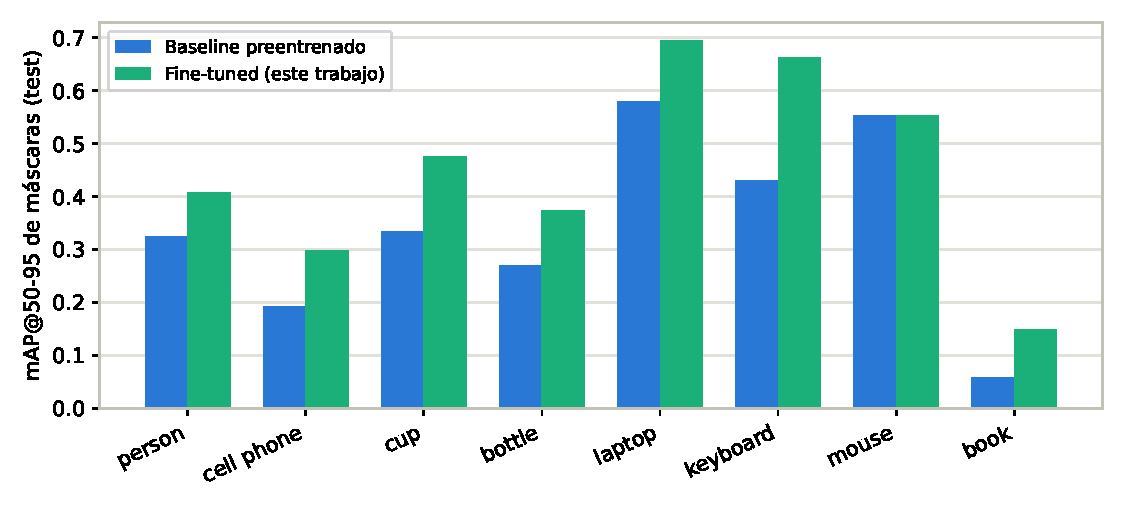
\includegraphics[width=0.85\textwidth]{baseline_vs_finetuned.pdf}
  \caption{Comparación imparcial por clase (mAP@50-95 de máscaras sobre COCO
  val2017): el modelo ajustado se aproxima al preentrenado en la mayoría de las
  clases, con paridad en \texttt{person} y \texttt{mouse}.}
  \label{fig:baseline}
\end{figure}

Los resultados revelan la magnitud del sesgo. Al pasar a datos no vistos, el
mAP@50-95 de máscaras del baseline \textbf{cae de 0,342 a 0,277}, mientras que
el del modelo ajustado apenas varía (de 0,246 a 0,236), coherente con que para
él ambas particiones son igualmente novedosas. En cajas, el baseline cae de
0,403 a 0,329 y el ajustado, de 0,292 a 0,275. Es decir: cerca de \textbf{dos
tercios de la brecha aparente} correspondían a la ventaja de fuga del baseline,
no a un defecto del modelo ajustado. Bajo la comparación justa la diferencia
global de máscaras se reduce a 0,041, y por clase el ajustado prácticamente
\textbf{iguala} al preentrenado en \texttt{person} ($-$0,008) y \texttt{mouse}
($-$0,007); la mayor diferencia persiste en \texttt{keyboard} ($-$0,115), la
clase con menos ejemplos de entrenamiento (116).

\textbf{Interpretación.} El modelo preentrenado es un baseline
excepcionalmente fuerte para este problema, por una razón de fondo: las ocho
clases son un \emph{subconjunto} de su vocabulario, y aprendió a reconocerlas a
partir de las 118.000 imágenes de COCO. Ajustar sobre 3.000 imágenes ---dos
órdenes de magnitud menos, y del mismo dominio--- no incorpora información nueva
y, con la cabeza de clasificación reinicializada, difícilmente pueda superarlo
en mAP; lo esperable es, precisamente, que lo iguale. El valor del ajuste fino
en este escenario no es un incremento de mAP sino la \textbf{especialización},
que se aprecia con claridad en el análisis cualitativo
(Sección~\ref{sec:cualitativo}).

\subsection{Ablación: efecto de congelar el \emph{backbone}}
\label{sec:ablacion}

La estrategia de congelar el \emph{backbone} (Sección~\ref{sec:metodo}) se
adoptó a partir de un experimento de ablación. La Tabla~\ref{tab:ablacion}
compara, sobre la partición de prueba, tres configuraciones: el modelo
preentrenado sin ajustar, un ajuste fino \emph{completo} (sin congelamiento, 60
épocas) y el ajuste con el \emph{backbone} congelado (150 épocas).

\begin{table}[H]
  \centering
  \small
  \caption{Ablación sobre la partición de prueba: efecto de la estrategia de
  ajuste en el mAP@50-95.}
  \label{tab:ablacion}
  \begin{tabular}{@{}lcc@{}}
    \toprule
    \textbf{Configuración} & \textbf{Cajas} & \textbf{Máscaras} \\
    \midrule
    Ajuste fino completo (sin congelar, 60 épocas) & 0,250 & 0,216 \\
    \textbf{Backbone congelado (150 épocas)} & \textbf{0,292} & \textbf{0,246} \\
    \bottomrule
  \end{tabular}
\end{table}

El ajuste fino completo, al reentrenar sin restricciones un clasificador
reinicializado sobre solo 3.000 imágenes, obtiene el peor resultado (0,216 de
máscaras). Congelar el \emph{backbone} ---preservando las representaciones de
COCO--- y extender el entrenamiento recupera cerca de un cuarto de la distancia
hacia el desempeño de referencia, y es la configuración que se reporta en el
resto del trabajo. La lección es que, cuando el vocabulario de destino es un
subconjunto del de preentrenamiento, un ajuste fino ingenuo puede \emph{degradar}
el modelo: preservar el \emph{backbone} es lo que convierte la transferencia en
una operación segura.

\subsection{Análisis cualitativo}
\label{sec:cualitativo}

Es aquí donde se vuelve tangible el verdadero aporte del ajuste fino. La
Figura~\ref{fig:cualitativo} contrasta las predicciones de ambos modelos sobre
el mismo lote de 16 imágenes de COCO~val2017. El baseline, con su vocabulario de
80 clases, dispersa detecciones entre numerosas categorías fuera del alcance del
sistema ---\texttt{refrigerator}, \texttt{oven}, \texttt{surfboard},
\texttt{horse}, \texttt{umbrella}, \texttt{pizza}, \texttt{skateboard},
\texttt{cow}, entre otras---; en la última imagen llega a etiquetar como
\texttt{cow} una escultura de vaca. El modelo ajustado, en cambio, concentra sus
detecciones \textbf{exclusivamente en las ocho clases de interés}: en la misma
escena detecta únicamente la \texttt{person} que aparece en la pantalla del
televisor. Para la aplicación objetivo ---que solo debe reconocer esas ocho
clases--- esta especialización es una ventaja práctica sustantiva, invisible a
la métrica de mAP por clase pero decisiva en el uso real, ya que suprime por
completo los falsos positivos de vocabulario. Se aprecian también los modos de
error residuales identificados en la matriz de confusión: personas pequeñas en
escenas concurridas y objetos poco frecuentes que no son detectados.

\begin{figure}[H]
  \centering
  \begin{subfigure}[b]{\textwidth}
    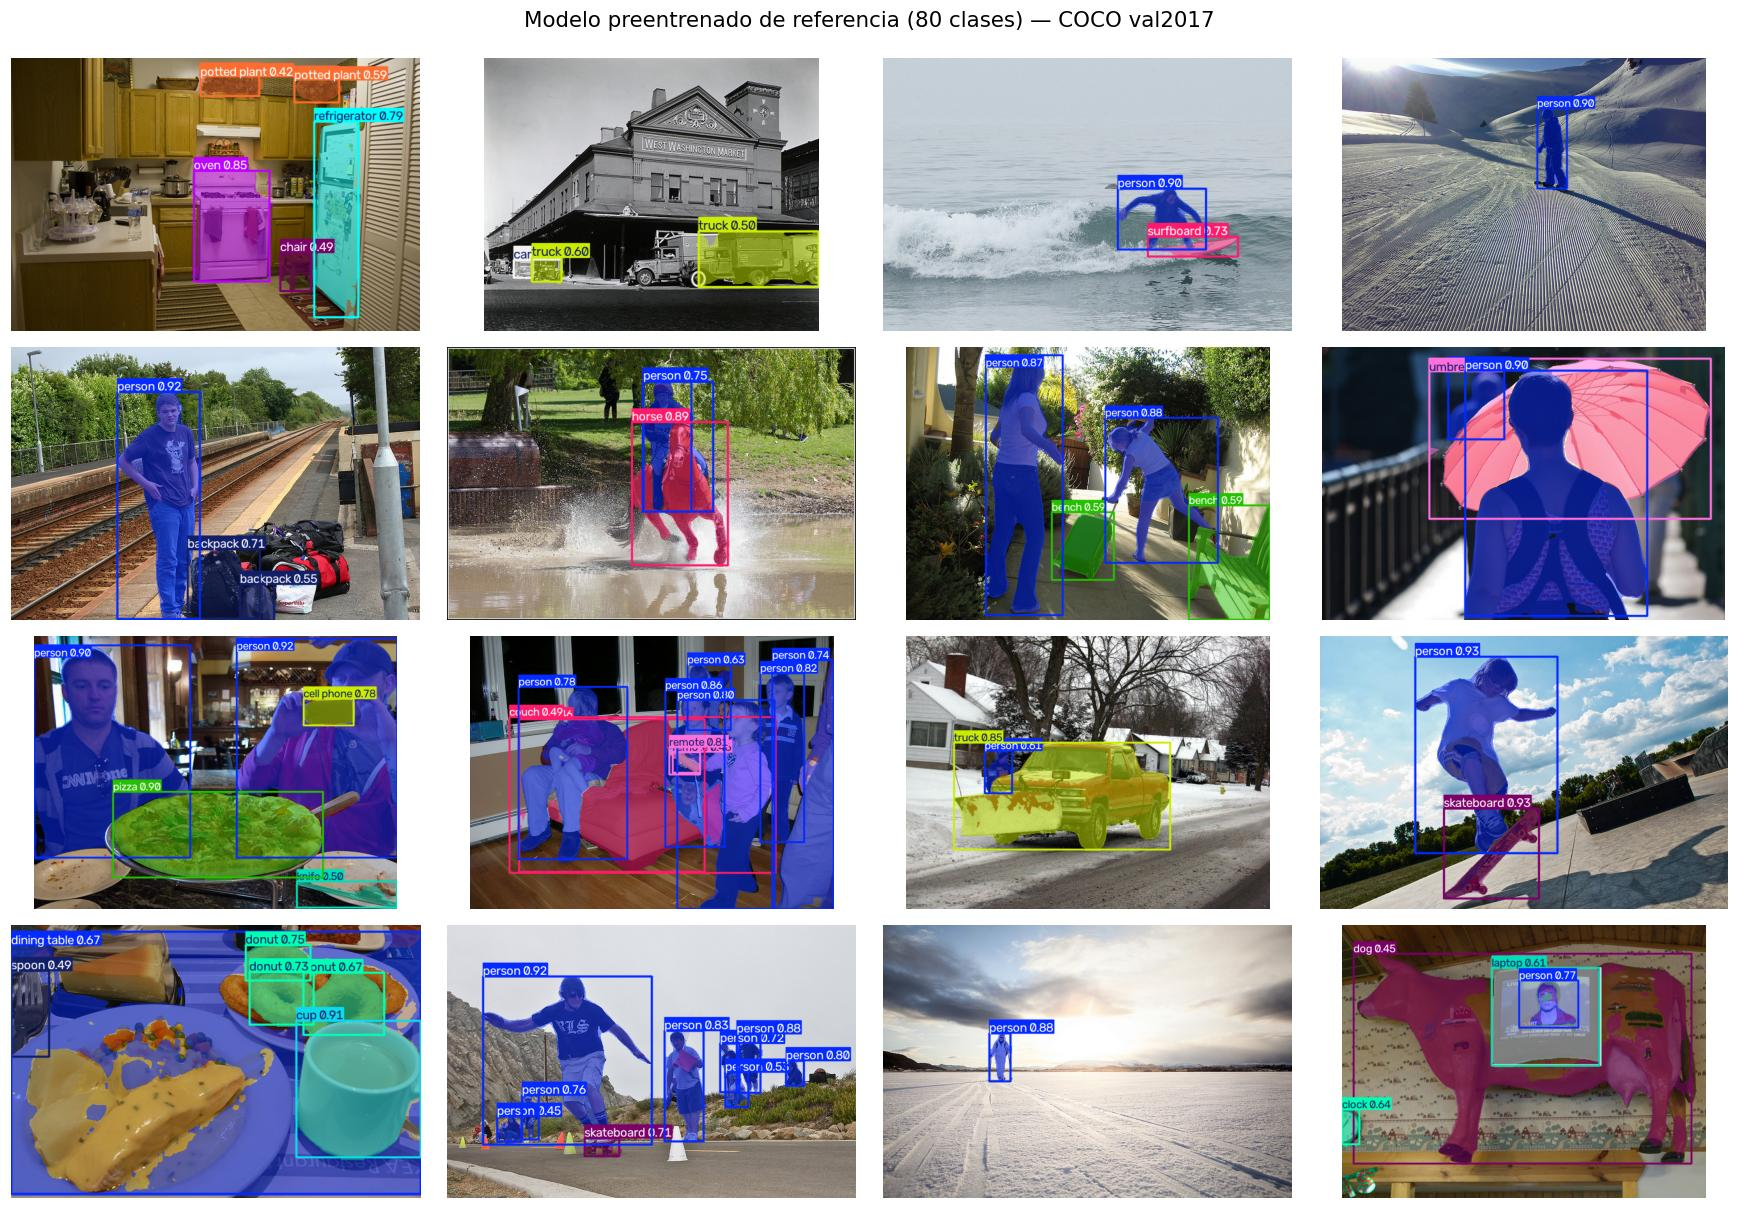
\includegraphics[width=\textwidth]{cualitativo_baseline.jpg}
    \caption{Modelo preentrenado de referencia (80 clases).}
  \end{subfigure}\\[1ex]
  \begin{subfigure}[b]{\textwidth}
    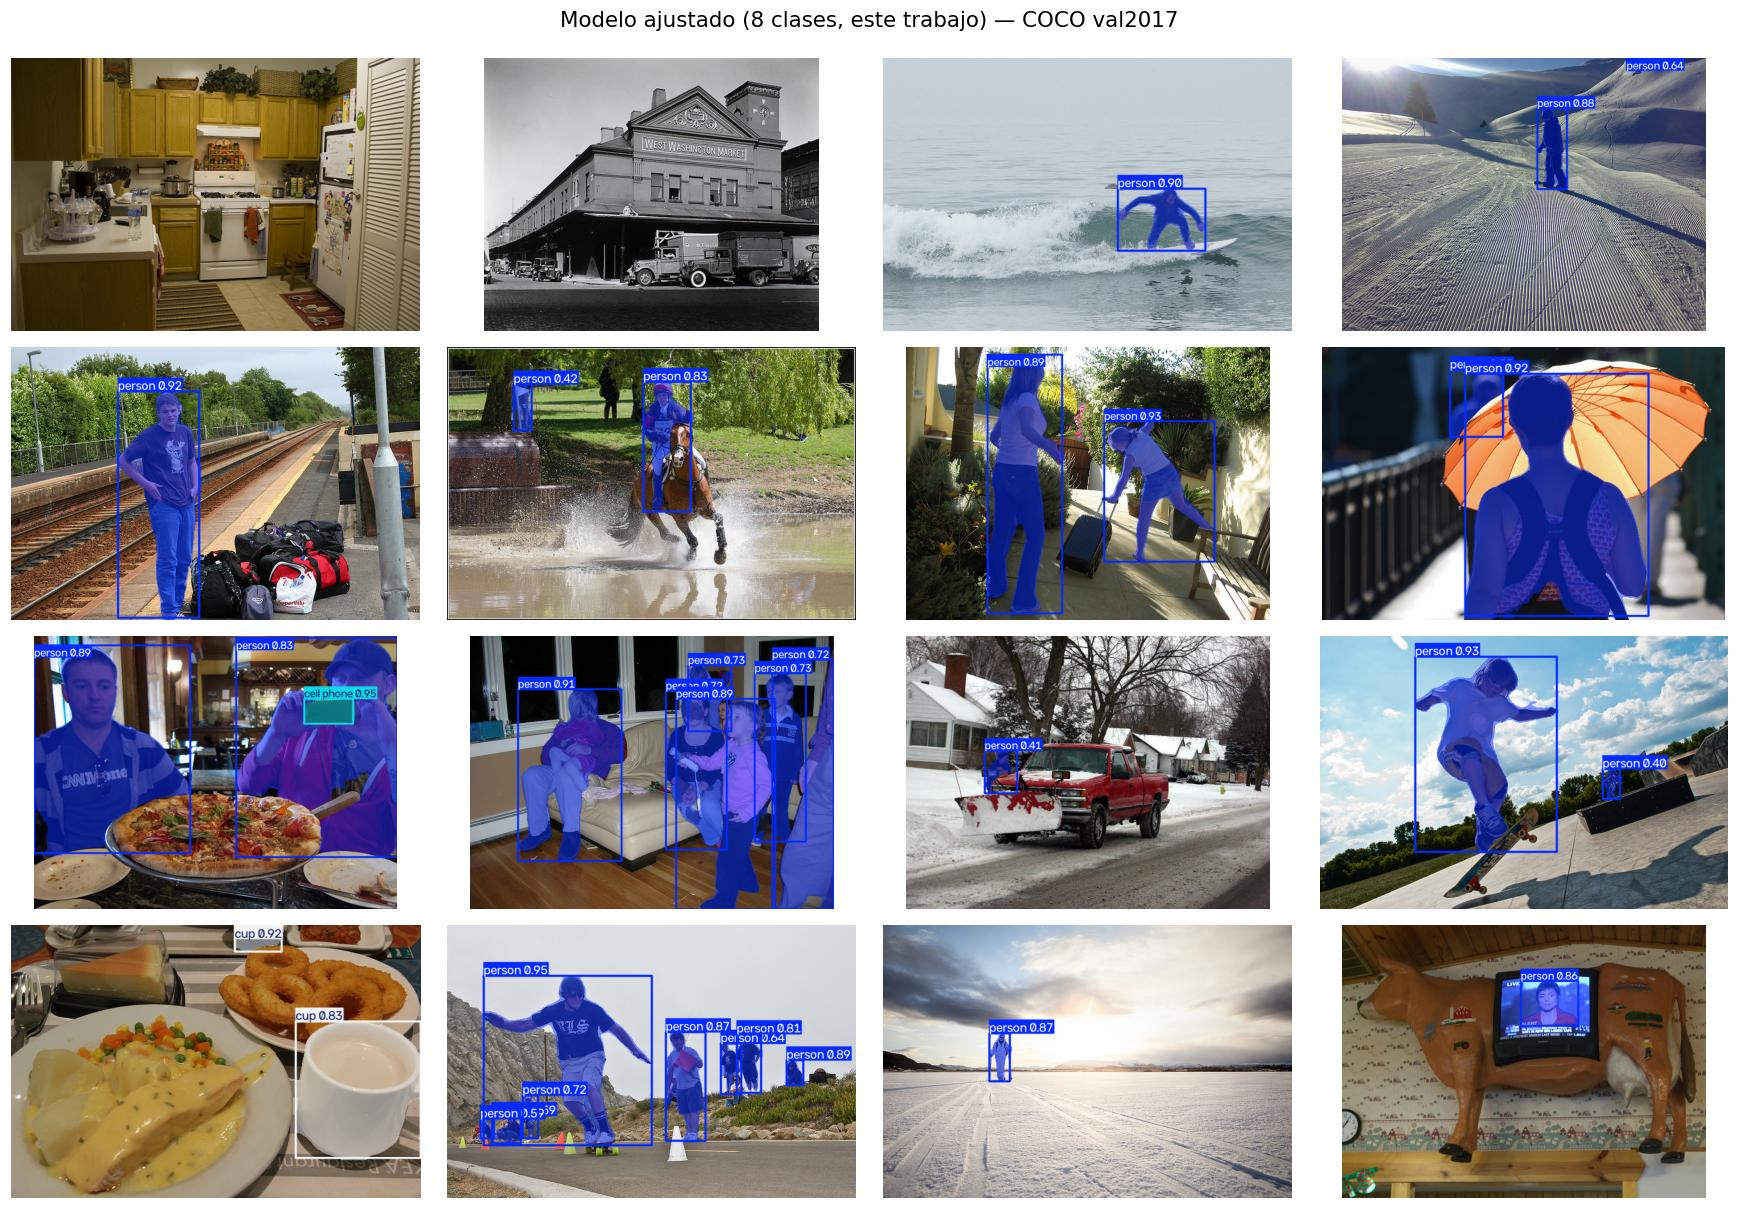
\includegraphics[width=\textwidth]{cualitativo_finetuned.jpg}
    \caption{Modelo ajustado (8 clases, este trabajo).}
  \end{subfigure}
  \caption{Predicciones de ambos modelos sobre el mismo lote de imágenes de
  COCO val2017 (umbral de confianza 0,4).}
  \label{fig:cualitativo}
\end{figure}

% ============================================================================
\section{Sistema de inferencia en tiempo real}
\label{sec:tiemporeal}

\subsection{Implementación}

El sistema de inferencia (\texttt{src/demo\_webcam.py}) captura video de una
cámara web ---o de un archivo--- mediante OpenCV, ejecuta el modelo sobre
cada cuadro y superpone en pantalla las cajas, las máscaras de instancia, las
etiquetas de clase con su confianza y la tasa de cuadros por segundo (FPS),
esta última suavizada con una media móvil exponencial para una lectura
estable. Los parámetros operativos (fuente de video, umbral de confianza,
resolución de inferencia) son configurables por línea de comandos. El
Código~\ref{lst:demo} muestra el núcleo del bucle de captura, inferencia y
visualización.

\begin{lstlisting}[style=py,caption={Núcleo del bucle de inferencia en tiempo
real (\texttt{src/demo\_webcam.py}): captura, predicción y superposición de
cajas y máscaras cuadro a cuadro.},label={lst:demo}]
modelo = YOLO(args.model, task='segment')     # pesos .pt o modelo OpenVINO
captura = cv2.VideoCapture(fuente)            # webcam (índice) o archivo de video

while True:
    ok, fotograma = captura.read()
    if not ok:
        break
    resultados = modelo.predict(fotograma, conf=args.conf,
                                imgsz=args.imgsz, verbose=False)
    anotado = resultados[0].plot()            # cajas + máscaras + etiquetas
    cv2.imshow(ventana, anotado)
    if cv2.waitKey(1) & 0xFF == ord('q'):     # 'q' para salir
        break
\end{lstlisting}

Dado que la computadora de demostración no dispone de GPU con CUDA, se evaluó
además la \textbf{optimización del modelo con OpenVINO} \cite{openvino}: los
pesos entrenados se exportaron al formato de representación intermedia de
Intel (\texttt{src/export\_openvino.py}, Código~\ref{lst:openvino}),
especializado para inferencia sobre CPU y gráficos integrados Intel.

\begin{lstlisting}[style=py,caption={Exportación de los pesos entrenados al
formato OpenVINO para acelerar la inferencia sobre CPU
Intel.},label={lst:openvino}]
modelo = YOLO('models/yolov8n_seg_best.pt')
ruta = modelo.export(format='openvino', imgsz=640, half=False)
\end{lstlisting}

\subsection{Desempeño medido}

La Tabla~\ref{tab:velocidad} resume las mediciones de latencia en las tres
configuraciones evaluadas. En el servidor, la rutina de validación reporta
5,1~ms por imagen ($\sim$198~FPS teóricos), holgadamente en tiempo real. En
la computadora personal (CPU Intel Core Ultra~5~226V), el modelo original en
formato PyTorch opera a 17~FPS, y la variante OpenVINO lo duplica hasta
35~FPS, superando el umbral convencional de tiempo real (24--30~FPS) sobre
hardware de consumo sin aceleración dedicada.

\begin{table}[H]
  \centering
  \small
  \caption{Velocidad de inferencia medida (resolución de entrada de 640
  píxeles).}
  \label{tab:velocidad}
  \begin{tabular}{@{}llcc@{}}
    \toprule
    \textbf{Plataforma} & \textbf{Formato del modelo} & \textbf{Latencia} & \textbf{FPS} \\
    \midrule
    Servidor, GPU RTX 5090 & PyTorch (\texttt{.pt}) & 5,1 ms/imagen & $\sim$198 \\
    PC personal, CPU Core Ultra 5 & PyTorch (\texttt{.pt}) & $\sim$59 ms/cuadro & 17 \\
    PC personal, CPU Core Ultra 5 & OpenVINO & $\sim$29 ms/cuadro & \textbf{35} \\
    \bottomrule
  \end{tabular}
\end{table}

La Figura~\ref{fig:webcam} muestra el sistema en operación sobre una escena
real de escritorio. En ambas capturas el modelo detecta y segmenta
correctamente los cinco objetos presentes (\texttt{person}, \texttt{book},
\texttt{mouse}, \texttt{bottle}), con máscaras que siguen el contorno de los
objetos ---incluida la silueta de la persona y el libro abierto sostenido en
la mano--- bajo la iluminación no controlada de la escena. El indicador de
FPS en pantalla evidencia la ganancia de la optimización: 17,2~FPS con el
modelo PyTorch frente a 35,6~FPS con OpenVINO, sobre la misma escena y el
mismo hardware.

\begin{figure}[H]
  \centering
  \begin{subfigure}[b]{0.49\textwidth}
    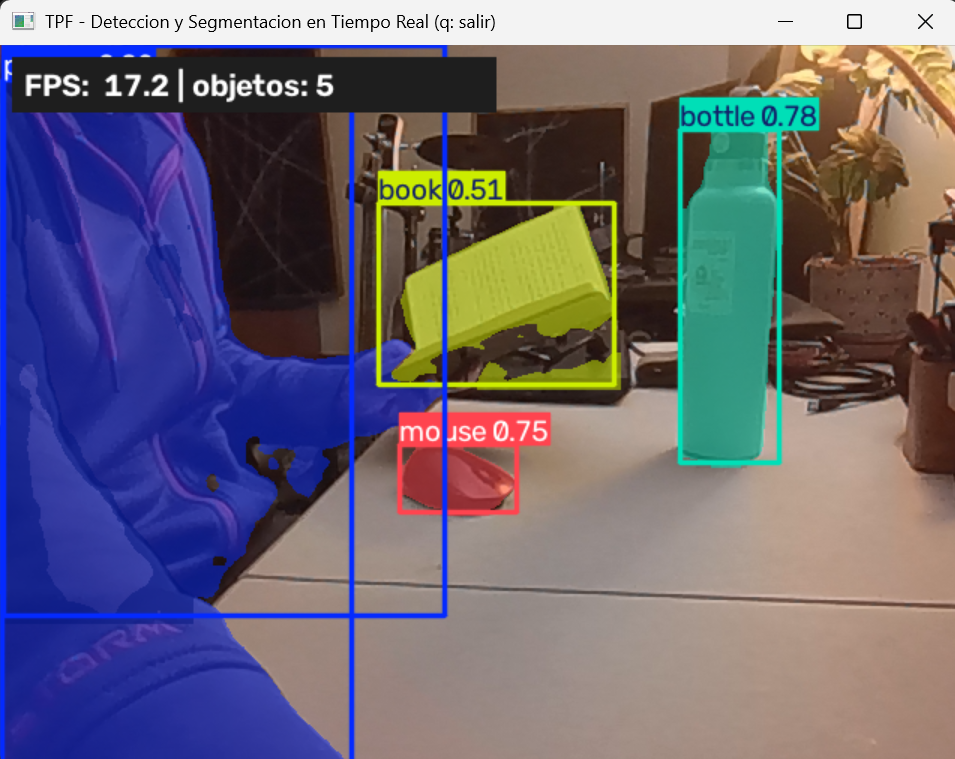
\includegraphics[width=\textwidth]{webcam_pt.png}
    \caption{Modelo PyTorch (\texttt{.pt}): 17,2 FPS.}
  \end{subfigure}
  \hfill
  \begin{subfigure}[b]{0.49\textwidth}
    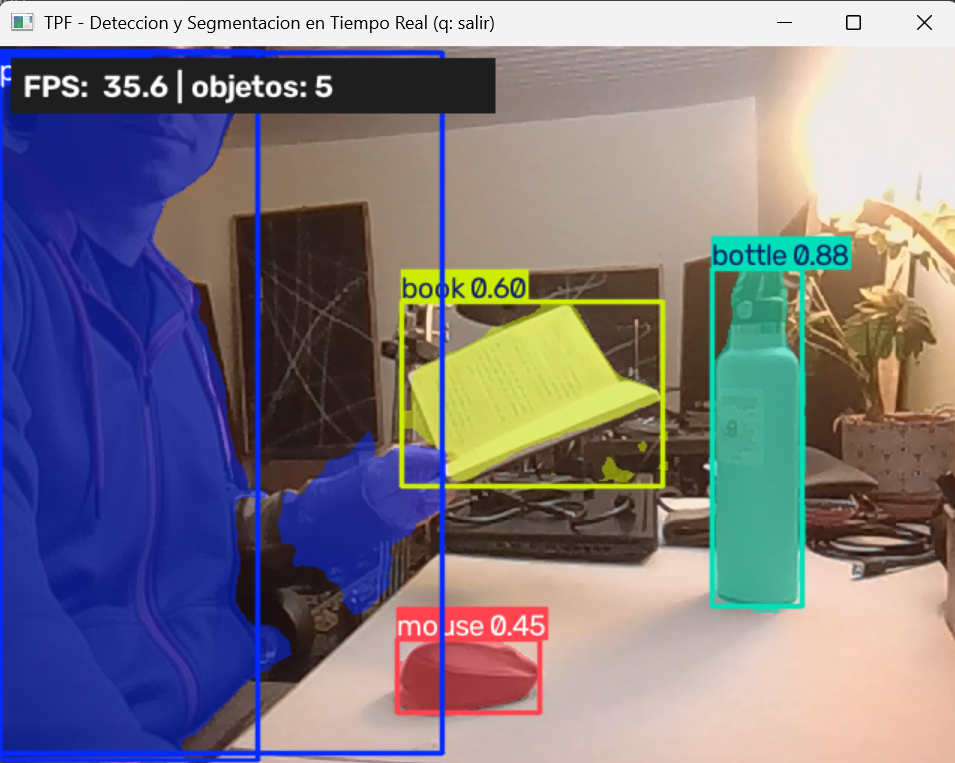
\includegraphics[width=\textwidth]{webcam_openvino.png}
    \caption{Modelo OpenVINO: 35,6 FPS.}
  \end{subfigure}
  \caption{Demostración del sistema en tiempo real sobre cámara web (CPU
  Intel Core Ultra 5 226V, sin GPU dedicada). Misma escena, cinco objetos
  detectados y segmentados en ambos casos.}
  \label{fig:webcam}
\end{figure}

% ============================================================================
\section{Prueba en servidor Hugging Face}
\label{sec:nube}

Además de la demostración local, la aplicación se \textbf{desplegó en un
servidor público} para que la inferencia pueda probarse en tiempo real desde
cualquier navegador, sin que quien la evalúe deba descargar ni instalar nada:
basta con abrir un enlace. Se empleó \textbf{Hugging Face Spaces} con una
interfaz \textbf{Gradio} \cite{gradio}; los pesos entrenados
(\texttt{yolov8n\_seg\_best.pt}) viajan dentro del propio repositorio del
Space, de modo que el modelo se ejecuta íntegramente en la nube.

La aplicación ofrece dos modos de uso: (i)~\emph{Imagen}, que corre el modelo
sobre una fotografía subida por el usuario y devuelve las cajas, las máscaras
de instancia y el recuento de objetos por clase; y (ii)~\emph{Webcam en vivo},
que ejecuta la inferencia cuadro a cuadro sobre la cámara del navegador, con
los controles de umbral de confianza y resolución de inferencia expuestos de
forma interactiva. La aplicación está disponible en:

\begin{center}
\url{https://huggingface.co/spaces/fedemoranf/TPF-DeepLearning-FedericoMoran}
\end{center}

La Figura~\ref{fig:huggingface} muestra la aplicación en funcionamiento sobre
el servidor. En la escena de escritorio de ejemplo, el modelo detecta y
segmenta correctamente cuatro de las ocho clases de interés ---\texttt{person}
(0,93), \texttt{bottle} (0,71), \texttt{cup} (0,57) y \texttt{cell phone}
(0,47)---, confirmando que el desempeño del modelo se traslada del entorno de
entrenamiento al despliegue en la nube.

\begin{figure}[H]
  \centering
  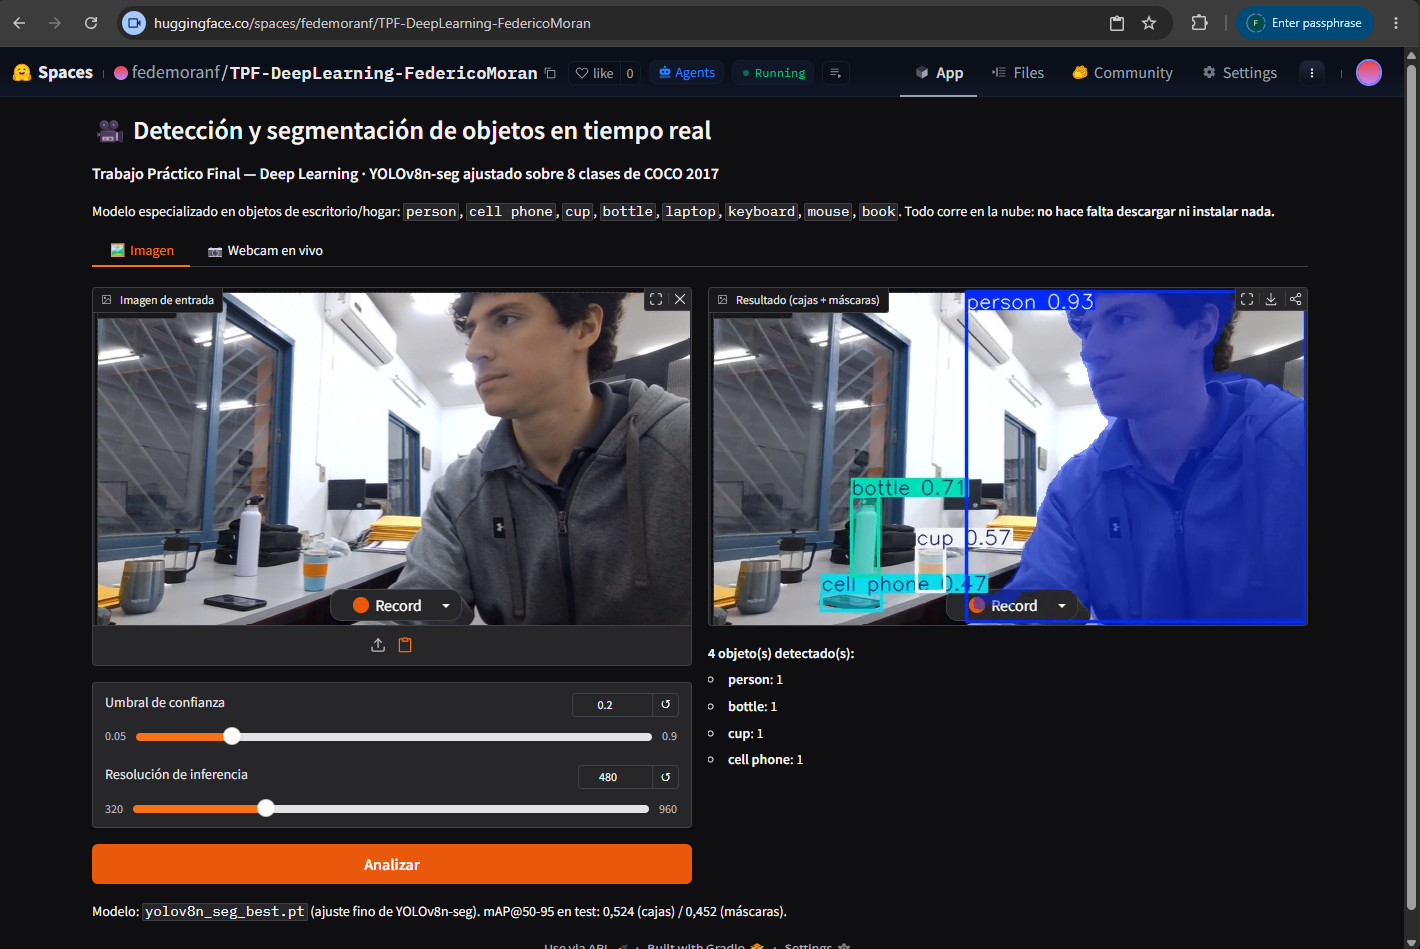
\includegraphics[width=\textwidth]{prueba_huggingface.png}
  \caption{Aplicación desplegada en Hugging Face Spaces (estado
  \emph{Running}), pestaña \emph{Imagen}. Sobre una escena de escritorio, el
  modelo detecta y segmenta cuatro clases objetivo (\texttt{person},
  \texttt{bottle}, \texttt{cup} y \texttt{cell phone}) con umbral de confianza
  0,2 y resolución de inferencia de 480~píxeles.}
  \label{fig:huggingface}
\end{figure}

% ============================================================================
\section{Conclusiones}
\label{sec:conclusiones}

Se desarrolló un sistema completo de visión por computadora que cubre el ciclo
íntegro de un proyecto de aprendizaje profundo aplicado: construcción de un
conjunto de datos supervisado (5.000 imágenes y 23.363 instancias de COCO
2017, con conversión y saneamiento de anotaciones de segmentación), ajuste
fino de un modelo de segmentación de instancias YOLOv8n-seg, evaluación
rigurosa con las métricas estándar del área e implementación de la inferencia
en tiempo real sobre hardware de consumo. Del trabajo se extraen las
siguientes conclusiones:

\begin{enumerate}
  \item \textbf{La evaluación rigurosa es tan determinante como el modelo
  mismo.} Se identificaron y corrigieron \emph{dos} fuentes de sesgo optimista:
  una fuga de datos en la propia partición ---la etiqueta de \emph{split} de
  origen de FiftyOne, controlada con \texttt{untag\_samples} y verificada con un
  \texttt{assert} sobre los archivos exportados--- y, más sutil, el hecho de que
  el modelo preentrenado de referencia fue entrenado sobre el mismo conjunto
  (COCO train2017) del que provienen las imágenes de prueba. Bajo una
  comparación imparcial sobre COCO val2017 ---datos no vistos por ninguno de los
  dos modelos--- la brecha aparente se reduce a la mitad y el modelo ajustado
  (0,236 de máscaras, 0,275 de cajas) resulta competitivo con el preentrenado
  (0,277 y 0,329), con paridad en varias clases. El experimento de ablación
  mostró que congelar el \emph{backbone} es lo que vuelve segura la
  transferencia: un ajuste fino completo, con la cabeza reinicializada,
  \emph{degrada} el modelo.
  \item \textbf{Cuando el vocabulario de destino es un subconjunto del de
  preentrenamiento, el aporte del ajuste fino es la especialización, no el
  mAP.} El preentrenado ya aprendió las ocho clases sobre 118.000 imágenes, de
  modo que 3.000 imágenes del mismo dominio no pueden superarlo en mAP. Lo que
  sí logra el ajuste, con claridad en el análisis cualitativo, es suprimir por
  completo los falsos positivos de las 72 categorías fuera de alcance, una
  ventaja decisiva para la aplicación objetivo.
  \item \textbf{El desempeño por clase está gobernado por las características
  visuales y la calidad de anotación de cada categoría.} Los objetos rígidos y
  poco ocluidos (\texttt{laptop}, \texttt{mouse}) superan 0,51 de mAP@50-95 de
  cajas, mientras que \texttt{book} ---instancias pequeñas, apiladas y de
  anotación ambigua en COCO--- queda en 0,051. La matriz de confusión muestra
  que el error dominante no es la confusión entre clases (máximo 0,03) sino la
  omisión de instancias pequeñas u ocluidas, lo que señala que el margen de
  mejora está en el \emph{recall} y no en la discriminación.
  \item \textbf{La segmentación de instancias en tiempo real es viable sobre
  una CPU de consumo.} La variante nano de YOLOv8-seg, exportada a OpenVINO,
  alcanzó 35~FPS sostenidos en una computadora personal sin GPU dedicada
  ---el doble que el formato PyTorch original---, validando la combinación de
  una arquitectura compacta con optimización específica del hardware de
  despliegue como estrategia para llevar modelos de segmentación a
  aplicaciones interactivas.
  \item \textbf{El pipeline resultó reproducible de extremo a extremo}: la
  selección de datos, las particiones y el entrenamiento están gobernados por
  semillas fijas y controles de integridad, y la demostración en vivo confirmó
  que el desempeño cuantitativo medido sobre COCO se traslada a escenas reales
  no controladas, con máscaras que siguen fielmente el contorno de los objetos.
\end{enumerate}

\vspace{1.5em}
\noindent\textbf{Anexos.} Acompañan a este informe los notebooks ejecutados
del pipeline (\texttt{01\_dataset}, \texttt{02\_entrenamiento},
\texttt{03\_evaluacion}), el código fuente del sistema de inferencia
(\texttt{src/}) y los pesos del modelo entrenado
(\texttt{models/yolov8n\_seg\_best.pt}).

% ============================================================================
\begin{thebibliography}{9}

\bibitem{lin2014coco}
T.-Y. Lin, M. Maire, S. Belongie, J. Hays, P. Perona, D. Ramanan,
P. Dollár y C. L. Zitnick,
``Microsoft COCO: Common Objects in Context'',
en \emph{Proc. European Conference on Computer Vision (ECCV)}, 2014.

\bibitem{jocher2023yolov8}
G. Jocher, A. Chaurasia y J. Qiu,
``Ultralytics YOLOv8'', 2023.
Disponible en: \url{https://github.com/ultralytics/ultralytics}

\bibitem{bolya2019yolact}
D. Bolya, C. Zhou, F. Xiao y Y. J. Lee,
``YOLACT: Real-time Instance Segmentation'',
en \emph{Proc. IEEE/CVF International Conference on Computer Vision (ICCV)}, 2019.

\bibitem{redmon2016yolo}
J. Redmon, S. Divvala, R. Girshick y A. Farhadi,
``You Only Look Once: Unified, Real-Time Object Detection'',
en \emph{Proc. IEEE Conference on Computer Vision and Pattern Recognition
(CVPR)}, 2016.

\bibitem{moore2020fiftyone}
B. E. Moore y J. J. Corso,
``FiftyOne'', GitHub, 2020.
Disponible en: \url{https://github.com/voxel51/fiftyone}

\bibitem{loshchilov2019adamw}
I. Loshchilov y F. Hutter,
``Decoupled Weight Decay Regularization'',
en \emph{Proc. International Conference on Learning Representations (ICLR)}, 2019.

\bibitem{openvino}
Intel Corporation,
``OpenVINO Toolkit: Open-source toolkit for optimizing and deploying AI
inference''.
Disponible en: \url{https://docs.openvino.ai}

\bibitem{gradio}
A. Abid, A. Abdalla, A. Abid, D. Khan, A. Alfozan y J. Zou,
``Gradio: Hacia una infraestructura de aprendizaje automático accesible para
cualquiera'', 2019.
Disponible en: \url{https://www.gradio.app}

\end{thebibliography}

\end{document}
